\documentclass[12pt, openright, a4paper, brazil, english, french, spanish, bibjustif, openany, oneside]{abntex2}

\usepackage{cmap}				% Mapear caracteres especiais no PDF
\usepackage{ifthen}				% Mapear caracteres especiais no PDF
\usepackage{setspace}				% Mapear caracteres especiais no PDF
\usepackage{lmodern}		
\usepackage[T1]{fontenc}	
\usepackage[utf8]{inputenc}
\usepackage{lastpage}
\usepackage{enumitem}	
\usepackage{indentfirst}	
\usepackage{color}			
\usepackage{graphicx}
\usepackage[table]{xcolor}
\usepackage{tabularx}
\usepackage{booktabs}
\usepackage{enumerate}		
\usepackage{microtype} 		
\usepackage{multicol}
\usepackage{multirow}
\usepackage{lipsum}
\usepackage{booktabs}				
\usepackage{bold-extra}				% Mapear caracteres especiais no PDF
\usepackage[final]{pdfpages}
\usepackage{float}

%aumentei a próxima linha
\usepackage{verbatim}

% \usepackage{subfig}
\usepackage{subcaption}


\usepackage[brazilian,hyperpageref]{backref}	 % Paginas com as citações na bibl
\usepackage[alf]{abntex2cite}	% Citações padrão ABNT

\usepackage{caption}


\newtheorem{teo}{Teorema}
	 
%
%\titulo{Usando o Scratch como ferramenta interdisciplinar através da programação}
%\autor{Sérgio Luís Soares Almeida \\ Matrícula 18/0006410}
%\local{Brasília}
%\data{2019}
%\instituicao{%
%  Universidade de Brasília -- UnB
%  \par
%  Departamento de Matemática
%  \par
% PROFMAT}
%\tipotrabalho{Estudo de Artigo}

%\definecolor{black}{RGB}{0.0,0.0,0.0}


%\makeatletter

%\preambulo{Scratch no ensino de Matemática}

%\hypersetup{pdftitle={\@title}, pdfauthor={\@author}, pdfsubject={\imprimirpreambulo}, pdfcreator={LaTeX with abnTeX2}, pdfkeywords={abnt}{latex}{abntex}{abntex2}{relatório técnico}, colorlinks=true, linkcolor=black, citecolor=black, filecolor=black, urlcolor=black, bookmarksdepth=4}
%\makeatother

%\setlength{\parindent}{1.3cm}


%\setlength{\parskip}{0.2cm}  


%\makeindex

%=============================================================================================
%teste de apendice
\renewcommand\appendixname{APÊNDICE}
\renewcommand\appendixpagename{APÊNDICE}
%=============================================================================================


%informações do título

\titulo{Usando o \textit{Scratch} como ferramenta interdisciplinar através da programação}
\autor{Sérgio Luís Soares Almeida}
\local{Brasília}
\data{\the\year}
\orientador[Orientadora:]{Profa. Dra. Tatiane da Silva Evangelista}
\coorientador{}
\instituicao{%
  Universidade de Brasília - UnB
  \par
  Departamento de Matemática - MAT
  \par
  PROFMAT - SBM}
\tipotrabalho{Dissertação de Mestrado}
% O preambulo deve conter o tipo do trabalho, o objetivo, 
% o nome da instituição e a área de concentração 
\preambulo{Dissertação apresentada ao Departamento de Matemática da Universidade de Brasília, como parte dos requisitos do Programa de Mestrado Profissional em Matemática em Rede Nacional - PROFMAT, para obtenção do grau de Mestre.}


%Novas configurações enviadas pelo Vinícius

\makeatletter
\newcommand*{\textoverline}[1]{$\overline{\hbox{#1}}\m@th$}
\makeatother
% ---
% Configurações do pacote backref
% Usado sem a opção hyperpageref de backref
\renewcommand{\backrefpagesname}{Citado na(s) página(s):~}
% Texto padrão antes do número das páginas
\renewcommand{\backref}{}
% Define os textos da citação
\renewcommand*{\backrefalt}[4]{
	\ifcase #1 %
		Nenhuma citação no texto.%
	\or
		Citado na página #2.%
	\else
		Citado #1 vezes nas páginas #2.%
	\fi}%
% ---

\renewcommand{\imprimircapa}{%
  \begin{capa}%
    \center
    \begin{minipage}[t][1cm][c]{0.2\textwidth}
        
\includegraphics[scale=0.6,keepaspectratio=true]{unb.png}
    \end{minipage}
    \begin{minipage}[t][1cm][c]{0.5\textwidth}
        \begin{center}
        Universidade de Brasília \\
        Instituto de Ciências Exatas \\
        Departamento de Matemática \\
        Programa de Mestrado Profissional\\
        em Matemática em Rede Nacional
        \end{center}
    \end{minipage}
    \begin{minipage}[t][1cm][c]{0.2\textwidth}
        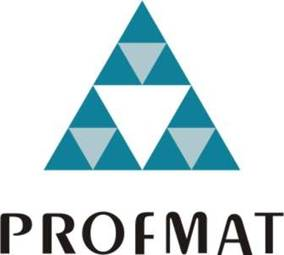
\includegraphics[scale=0.6,keepaspectratio=true]{profmat.jpg}
    \end{minipage}

    \vspace*{1cm}

    \vfill
    \begin{center}
    \ABNTEXchapterfont\bfseries\LARGE\imprimirtitulo
    \end{center}
    \vfill

    {\ABNTEXchapterfont\large\imprimirautor}

    \vspace*{2cm}

    \large\imprimirlocal

    \large\imprimirdata

    \vspace*{1cm}
  \end{capa}
}

\newcounter{obmepquestion}

\newenvironment{enunciado}
{
    \stepcounter{obmepquestion}
    \bfseries
}
{
}

\newenvironment{analise}[8]
{
    \vspace{0.2in}
    \noindent
    \begin{minipage}[c][4cm][c]{0.55\textwidth}
        
    \begin{small}
    \begin{center}
    \bfseries{\scshape{Análise do Item \arabic{obmepquestion}}}
    \end{center}
    \end{small}

    \begin{tiny}
    \begin{tabular}{cccccc}
        \toprule
        \rowcolor{blue!20}
        Questão & Gabarito & Dificuldade & \multicolumn{2}{c}{Índice D} &
            Bisserial \\
        #1 & \multicolumn{2}{c}{#2} & #3 \\
        \rowcolor{blue!20}
        \multicolumn{3}{c}{Acerto: 27\% maiores notas} &
        \multicolumn{3}{c}{Acerto: 27\% menores notas} \\
        \multicolumn{3}{c}{#4} &
        \multicolumn{3}{c}{#5} \\
        \rowcolor{blue!20}
        $r_b(A)$ & $r_b(B)$ & $r_b(C)$ & $r_b(D)$ & $r_b(E)$ & $r_b()$ \\ 
        #6 \\
        \rowcolor{blue!20}
        $p(A)$ & $p(B)$ & $p(C)$ & $p(D)$ & $p(E)$ & $p()$ \\ 
        #7 \\
        \bottomrule
    \end{tabular}
    \end{tiny}
    \end{minipage}
    \begin{minipage}[c][4cm][c]{0.45\textwidth}
        \includegraphics[scale=0.25,keepaspectratio=true]{#8}
    \end{minipage}
}
{
    \vspace{0.2in}
}


\newcommand{\alternativas}[6]
{
    \vspace{0.2in}
    \noindent
    \begin{minipage}[t][1cm][c]{0.5\textwidth}
    \begin{flushleft}
    \begin{enumerate}[itemsep=-2mm, label=\Alph*)]
        \item #1
        \item #2
        \item #3
        \item #4
        \item #5
    \end{enumerate}
    \end{flushleft}
    \end{minipage}
    \begin{minipage}[t][1cm][c]{0.5\textwidth}
    \ifthenelse{\equal{#6}{}}{}{
        \includegraphics[scale=0.6,keepaspectratio=true]{#6}
    }
    \end{minipage}
    \vspace{0.5in}
}

% ---
% Configurações de aparência do PDF final

% alterando o aspecto da cor azul
\definecolor{blue}{RGB}{41,5,195}

% informações do PDF
\makeatletter

\hypersetup{
     	%pagebackref=true,
		pdftitle={\@title}, 
		pdfauthor={\@author},
    	pdfsubject={\imprimirpreambulo},
	    pdfcreator={LaTeX with abnTeX2},
		pdfkeywords={abnt}{latex}{abntex}{abntex2}{trabalho acadêmico}, 
		colorlinks=true,       		% false: boxed links; true: colored links
    	linkcolor=black,          	% color of internal links
    	citecolor=black,        		% color of links to bibliography
    	filecolor=black,      		% color of file links
		urlcolor=black,
		bookmarksdepth=4
}
\makeatother
% --- 

% --- 
% Espaçamentos entre linhas e parágrafos 
% --- 

% O tamanho do parágrafo é dado por:
\setlength{\parindent}{1.3cm}

% Controle do espaçamento entre um parágrafo e outro:
\setlength{\parskip}{0.2cm}  % tente também \onelineskip

\begin{document}






\selectlanguage{brazil}


\frenchspacing 
\imprimircapa
\imprimirfolhaderosto*
\ABNTEXchapterfont

%novos elementos do documento
% FICHA CATALOGRÁFICA

\begin{fichacatalografica}
	\vspace*{\fill}					% Posição vertical
	\hrule							% Linha horizontal
	\begin{center}					% Minipage Centralizado
	\begin{minipage}[c]{12.5cm}		% Largura

	\imprimirautor
	
	\hspace{0.5cm} \imprimirtitulo  / \imprimirautor. --
	\imprimirlocal, \imprimirdata-
	
	\hspace{0.5cm} \pageref{LastPage} p. : il. (algumas color.) ; 30 cm.\\
	
	\hspace{0.5cm} \imprimirorientadorRotulo~\imprimirorientador\\
	
	\hspace{0.5cm}
	\parbox[t]{\textwidth}{\imprimirtipotrabalho~--~\imprimirinstituicao,
	\imprimirdata.}\\
	
	\hspace{0.5cm}
		1. \textit{Scratch}.
		2. Interdisciplinar.
		3. Pensamento Computacional.
		4. Linguagem de Programação.
		I. Prof Dra Tatiane da Silva Evangelista.
		II. Universidade de Brasília.
		III. PROFMAT - SBM.
		IV. Título Usando o \textit{Scratch} como ferramenta interdisciplinar através da programação\\ 			
	
	\hspace{8.75cm} \\ %{?CDU XYZ 02:141:005.7?} 
	
	\end{minipage}
	\end{center}
	\hrule
\end{fichacatalografica}

% FOLHA DE APROVAÇÃO

\begin{folhadeaprovacao}

\begin{center}
 Universidade de Bras\'ilia \\
 Instituto de Ci\^encias Exatas \\
 Departamento de Matem\'atica
\end{center}
\begin{center}
    \vspace{0.3cm}
 \LARGE{\textbf{\imprimirtitulo}}
    \vspace{0.3cm}
\end{center}
\begin{center}
 por \\
    \vspace{0.5cm}
 \LARGE{\textbf{\imprimirautor}}
\end{center}

    \vspace{0.5cm}
\noindent Disserta\c c\~ao apresentada ao Departamento de Matem\'atica da Universidade de Bras\'ilia,
como parte dos requisitos do Programa de Mestrado Profissional em Matem\'atica em Rede 
Nacional - PROFMAT, para obten\c c\~ao do grau de 
\begin{center}
    \vspace{0.2cm}
 \LARGE{\textbf{MESTRE}}\\
    \vspace{0.5cm}
 Bras\'ilia, 28 de Julho de 2020 % NÃO ESQUECER DE ARRUMAR A DATA
\end{center}

    \vspace{1.5cm}
\noindent {Comiss\~ao Examinadora:}

\vspace*{8mm}

\textoverline{\phantom{xxxxxxx} \imprimirorientador - MAT/UnB (Orientadora)\phantom{xxxxxxx}  }

\vspace*{1cm}

\textoverline{\phantom{xxxxxxx}  Prof. Dr. Matheus Bernardini de Souza - MAT/UnB (Membro Interno)\phantom{xxxxx} }

\vspace*{1cm}

\textoverline{\phantom{xxxxxxx}  Prof. Dr. Ronni Geraldo G. de Amorim - FGA/UnB (Membro Externo)\phantom{xxxxx}  }

\vspace*{1cm}

\vspace*{1cm}

\end{folhadeaprovacao}

%folha dedicatória

\begin{dedicatoria}
   \vspace*{\fill}
   \centering
   \noindent
    \textit{Dedico esse trabalho primeiramente a Deus, que sempre esteve ao meu lado nos momentos de angústia, à minha mãe, Maria de Jesus Soares, aos meus irmãos, Liana Soares e Marcelo Soares e ao meu filho Gabriel Rodrigues que sempre me incentivaram e ainda me incentivam a continuar na vida acadêmica.}\vspace*{\fill}
    
\end{dedicatoria}

%folha agradecimentos

\begin{agradecimentos}

Agradeço em primeiro lugar a Deus por ter me abençoado e iluminado o meu caminho, me mostrando quais as escolhas corretas e como a vida é maravilhosa. Agraceço a minha mãe, \textit{Maria de Jesus Soares}, o meu maior exemplo de determinação. Agradeço aos meus irmãos \textit{Marcelo Soares} e \textit{Liana Soares} por sempre me apoiarem e me incentivarem.

Agradeço ao meu filho, \textit{Gabriel Rodrigues}, que sempre esteve ao meu lado, me incentivando, me apoiando e me trazendo muita alegria. Obrigado por estar sempre presente em todos os momentos da minha vida.

Agradeço a todos os amigos da turma do PROFMAT 2018. Sempre lembrarei dos momentos maravilhosos que passamos juntos.

Agradeço à minha professora e orientadora, professora Tatiane, pela sua amizade, pelos conselhos, por ter acreditado no meu potencial e nesse trabalho.

Agradeço aos meus amigos \textit{Clébia}, \textit{Cláudio}, \textit{Douglas}, \textit{Fabiano}, \textit{Mayco}, \textit{Wagner} e \textit{Rodrigo} por me mostrarem como a união pode superar qualquer dificuldade e como o estudo em grupo é essencial na vida acadêmica.

Agradeço a todos que sempre me acompanharam e sempre torceram por mim.

\end{agradecimentos}

%folha epigrafe

\begin{epigrafe}
    \vspace*{\fill}
	\begin{flushright}
		\textit{\lq\lq Educar verdadeiramente não é ensinar fatos novos ou enumerar fórmulas prontas, mas sim preparar a mente para pensar \rq\rq\\ Albert Einstein}
	\end{flushright}
\end{epigrafe}

%folha resumo

\begin{resumo}

O computador ainda é utilizado na Educação apenas como meio de reprodução de atividades que anteriormente eram desenvolvidas por outros meios de comunicação como, por exemplo, exposição e criação de resumos, reprodução de trabalhos escolares e citação de trechos de livros através de \textit{blogs} e \textit{sites}. Os conhecimentos em computação podem ser usados de maneira que os alunos não sejam apenas usuários das Tecnologias Digitais de Comunicação e de Informação, mas que também possam ser produtores de tecnologia. Com base na teoria do Pensamento Computacional, a inserção da computação na educação pode ser fator determinante na construção de novos conhecimentos e habilidades advindas do raciocínio lógico e da abstração de problemas. Desta forma, o \textit{Scratch}, uma plataforma de programação idealizada por Mitchel Resnick para crianças a partir de 08 anos de idade e criado em 2007 pelo MIT (Instituto de Tecnologia de Massachussets), pode ser usado para os estudos de conteúdos interdisciplinares com a inserção do estudo da computação em sala de aula e na construção de Objetos Digitais de Aprendizagem para a Educação Básica. Assim, em parceria com o Centro de Referência em Tecnologia Educacional do Recanto das Emas no Distrito Federal, foi oferecido uma formação do \textit{Scratch} para professores da rede pública de ensino para incentivá-los a usar essa plataforma de maneira dinâmica e intuitiva. Em razão disso, o objetivo desse trabalho foi relatar este curso e observar como os professores e alunos podem desenvolver projetos usando a computação e quais os benefícios que esse uso e esses projetos podem ajudar na relação ensino-aprendizagem e assim percebeu-se que o \textit{Scratch} não só é uma ferramenta capaz de ser usada de forma interdisciplinar como também oferece condições para uma mudança no processo de aprendizagem e nas relações entre professores e alunos, transformando o conhecimento em uma construção contínua.


 \vspace{\onelineskip}
    
 \noindent
 \textbf{Palavras-chaves}: Interdisciplinar. Computação. Educação. \textit{Scratch}.
\end{resumo}

%folha abstract

\begin{resumo}[Abstract]
 \begin{otherlanguage*}{english}

Computers are still used in Education only as a means of reproducing activities that were previously carried out by other means of communication, such as, for example, displaying and creating abstracts, reproducing schoolwork and citing excerpts from books through blogs and websites. Computer skills can be used in such a way that students are not only users of Digital Communication and Information Technologies, but can also be technology producers. Based on the Computational Thinking theory, the insertion of computing in education can be a determining factor in the construction of new knowledge and skills arising from logical reasoning and problem abstraction. Thereby, Scratch, a programming platform designed by Mitchel Resnick for children from 08 years of age and created in 2007 by MIT (Massachusetts Institute of Technology), can be used for the study of interdisciplinary content with the insertion of study of computing in the classroom and in the construction of Digital Learning Objects for Basic Education. Thus, in partnership with the Educational Technology Reference Center of Recanto das Emas in the Federal District, Scratch training was offered to public school teachers to encourage them to use this platform in a dynamic and intuitive way. As a result, the objective of this work was to report the course in question and observe how teachers and students can develop projects using computing, in addition to extolling its benefits in relation to the teaching learning process. Thereby, it was realized that Scratch is not only a tool capable of being used in an interdisciplinary way, but also offers conditions for a change in the learning process and in the relationships between teachers and students, transforming knowledge into a continuous construction.

  \vspace{\onelineskip}
 
   \noindent 
 \textbf{Key-words}: Interdisciplinary. Computing. Education. Scratch.
 \end{otherlanguage*}
\end{resumo}



%novas configurações de capa e contracapa
\pdfbookmark[0]{\listfigurename}{lof}
\listoffigures*
\cleardoublepage

\pdfbookmark[0]{\listtablename}{lot}
\listoftables*
\cleardoublepage

\pdfbookmark[0]{\contentsname}{toc}
\tableofcontents*
\cleardoublepage
% ----------------------------------------------------------
% ELEMENTOS TEXTUAIS
% ----------------------------------------------------------
\textual

%\ABNTEXchapterfont
%\pdfbookmark[0]{\contentsname}{toc}
%\tableofcontents*
%\cleardoublepage
%\textual

\chapter{Introdução}
% \addcontentsline{toc}{chapter}{Introdução}

As novas Tecnologias Digitais de Informação e de Comunicação causaram e ainda causam grandes transformações no trabalho, nas relações interpessoais e na sociedade em geral, mas essas transformações não são tão rápidas e tão profundas na educação, especialmente na educação básica. O computador, como ferramenta educacional, ainda é muito utilizado apenas como um meio de reprodução de atividades que já eram desenvolvidas anteriormente mudando apenas o meio de comunicação. A forma de apresentar os conteúdos e as aulas, em sua essência, progrediram pouco ou quase nada, com o professor ainda sendo o detentor do conhecimento e os alunos com o objetivo de reproduzir esses conhecimentos que agora podem ser pesquisados nos \textit{sites} e nos \textit{blogs} escritos ou indicados pelo professor.


O uso das tecnologias na educação não pode servir apenas a uma proposta onde o computador passe alguma instrução ao aluno mas, principalmente, crie oportunidades para que o estudante possa programar e criar. É necessária uma nova abordagem no ensino, de forma que o aluno possa ser independente, que saiba procurar, selecionar e resolver os problemas ao seu redor usando as informações disponíveis e, desta forma, aprendendo com as situações apresentadas em seu meio social e cultural. 

Nos últimos anos, alguns pesquisadores defendem que os conhecimentos em Computação sejam inseridos no ambiente escolar, dado que ``...são tão importantes para a vida na sociedade contemporânea quanto os conhecimentos básicos de Matemática, Filosofia, Física, dentre outras, assim como contar, abstrair, pensar, relacionar ou medir'' \cite{brac}. Em contrapartida, a linguagem de programação, acrescenta ao aluno um raciocínio lógico aguçado capaz de entender essas novas tecnologias não apenas como um mero usuário, mas como um indivíduo com a habilidade de modificar e criar novos conhecimentos que podem ser aplicados em sua vida acadêmica, em seu trabalho e em seu cotidiano.

Diante desse cenário, o \textit{Scratch} é uma ferramenta que propõe a introdução da linguagem de programação acessível e interdisciplinar dando a possibilidade ao aluno de criar seus próprios programas, jogos, histórias e apresentações e com a capacidade de desenvolver o raciocínio lógico de forma gradual e sistemática facilitando a resolução de problemas mais complexos e mais abrangentes.

Em parceria com o Centro de Referência em Tecnologia Educacional (CRTE) do Recanto das Emas - Distrito federal e sentindo também a necessidade de inserir o \textit{Scratch} na sala de aula com base no Currículo de Educação Básica, foi oferecido uma formação com duração de 21 horas diretas e 9 indiretas para professores da rede pública de ensino de diferentes formações acadêmicas e de diferentes modalidades e funções. Os CRTE são setores da Secretaria Estadual de Educação criados em todas as regiões administrativas do Distrito Federal que oferecem formações variadas e tem como principal atribuição contribuir para a melhoria da qualidade  do ensino e a operacionalização do Currículo de Educação Básica, por meio de implementação, acompanhamento e utilização pedagógica das Tecnologias Digitais de Informação e de Comunicação junto às unidades escolares da Rede Pública de Ensino do Distrito Federal. Desta forma pôde-se também estudar de que forma a programação através do \textit{Scratch} realmente contribui na aprendizagem e na compreensão dos conteúdos de forma interdisciplinar.

Outros objetivos inerentes aos estudos realizados nesse trabalho são:
\begin{itemize}


\item Analisar como o \textit{Scratch} contribui para a inserção de conteúdos referentes ao currículo escolar.
\item Observar como os professores, em suas determinadas áreas, conseguem utilizar os conceitos de linguagem de programação e algoritmos em sua prática pedagógica.
\item Observar, através de depoimentos dos professores e da apresentação dos trabalhos realizados pelos seus alunos, o desenvolvimento construtivista e construcionista gerado pela inserção do \textit{Scratch}.

\end{itemize}

Para um melhor entendimento, esse trabalho foi dividido de tal forma que um capítulo é destinado a apresentação dos estudos que servem de embasamento teórico para o curso, outro capítulo tem como objetivo apresentar o que é o \textit{Scratch} de forma geral e como ele foi criado e em mais um capítulo será explicado a metodologia do curso com a descrição dos estudos realizados em cada encontro e com os resultados obtidos e, após isto, apresenta-se a conclusão dos estudos realizados.




%- relação entre tecnologia e ensino
%- \textit{Scratch} para ajudar na utilização da lógica.
%O ensino é o ato ou processo de transmitir ou adquirir conhecimento,
%desenvolvendo nos interessados a capacidade de interpretação e julgamento das
%informações (Collins e Halverson, 2009). Em Toffler (1980) é relatado que a sociedade
%altera suas diretrizes com o passar do tempo, através do estilo familiar, de maneiras
%diferentes de realizar um dado trabalho, a política, e até mesmo a consciência das
%- facilitador da relação ensino-aprendizagem
%- desafios de como organizar o pensamento para resolução de problemas
%- Cursos CRTE
%- Quem foi envolvido
%- tdics na educação
%- importância do conhecimento da computação

%Nos últimos anos, vem surgindo um movimento de inserção da linguagem de progra-
%mação em sala de aula, defendida por alguns pesquisadores como uma nova disciplina, como
%Barichelo (2015, p. 26), que se justifica pelo fato de que o mercado de trabalho em áreas
%correlatas é grande e deve continuar aumentando, além de tratar de habilidades e conhecimentos
%cada vez mais presentes em todas as áreas.
%Por outro lado, há quem defenda a linguagem de programação na escola como uma
%ferramenta para o ensino dos conteúdos, como Batista et al. (2015, p. 351), que a veem como “um Objeto de Aprendizagem no ensino básico de uma forma multidisciplinar”.



\chapter{Referencial Teórico}

A sociedade não precisa mais esperar o horário fixo de um determinado programa, de um determinado noticiário, ou até mesmo de um jornal impresso ou de um livro, as novas Tecnologias Digitais de Informação e de Comunicação apresentam um novo modelo de espaço e tempo, proporcionando a qualquer pessoa a escolher qual o momento ideal para ter acesso a uma notícia, qual o melhor lugar para assistir a um filme ou série, qual o passatempo a ser acessado, desta forma cada indivíduo faz a sua programação em seu tempo e em seu espaço, acessando as notícias e as informações que lhes sejam interessantes e descartando o que não os interessa. Esse novo modelo de relação das novas Tecnologias Digitais de Informação e de Comunicação com o tempo e espaço ainda não foram totalmente assimiladas pela escola.

\begin{citacao}

``Estas tecnologias começam a afetar profundamente a educação. Esta sempre esteve e continua presa a lugares e tempos determinados: escola, salas de aula, calendário escolar, grade curricular''\cite{moran}.

\end{citacao}


A escola continua a ser uma instituição que, apesar do avanço nas Tecnologias Digitais de Informação e de Comunicação, continua com os mesmos conceitos de ensino focados no professor e no conteúdo tendo como finalidade principal o ensino em vez da aprendizagem. 

\begin{citacao}

``As tecnologias chegaram na escola, mas estas sempre privilegiaram mais o controle a modernização da infraestrutura e a gestão do que a mudança''\cite{moran}.

\end{citacao}

Ao mudar o foco do ensino para a aprendizagem, a escola deixa de ser o local exclusivo na construção do conhecimento e o aluno conquista autonomia como cidadão e como agente do próprio conhecimento levando em consideração as informações apresentadas, refletindo e relacionando-as ao tempo e espaço escolhidos. Neste processo, o professor deixa de ser o detentor do conhecimento e passa a ser o mediador da aprendizagem, com o papel de facilitador na organização e criação do conhecimento de forma sólida e multidisciplinar. 

\newpage

\section{Conexão: Construcionismo e Construtivismo}

% Começou-se a falar sobre o uso da linguagem de programação nas escolas assim que
% surgiram os primeiros computadores pessoais, sendo um dos precursores o Professor Seymour
% Papert (1980, p. 55), do Massachusetts Institute of Technology (MIT), que desenvolveu a lin-
% guagem de programação Logo.
% No Brasil, temos o Superlogo, um software gratuito que utiliza uma versão da lingua-
% gem Logo em português e foi desenvolvido pelo Núcleo de Informática Aplicada à Educação
% (Nied) da Universidade Estadual de Campinas (Unicamp). O objetivo do Superlogo é movimen-
% tar a figura de uma tartaruga utilizando orientações que são digitadas na janela de comandos.
% Os mais básicos deles se referem a movimentação no plano, mas as possibilidades são diversas.

%No entanto, dentre essas atividades, percebeu-se que vários conceitos matemáticos
%necessitam ser compreendidos para desenvolver os jogos e animações, surgindo então a
%ideia de desenvolver atividades de forma contextualizada e interdisciplinar, como forma
%de ajudá-los na aprendizagem de temas abordados em sala de aula.

Um dos primeiros a estudar e a defender o uso da linguagem de programação nas escolas foi o Professor Seymour Papert, do \textit{Massachusetts Institute of Technology} (MIT), através da linguagem LOGO. Ele percebeu que muitas escolas usam o computador para ensinar as crianças através de instruções e desta forma ``o computador está sendo usado para programar a criança'' \cite{papert}. Para ele

\begin{citacao}

``... é a criança que deve programar o computador e, ao fazê-lo, ela adquire um sentimento de domínio sobre um dos mais modernos e poderosos equipamentos tecnológicos e estabelece um contato íntimo com alguma das ideias mais profundas da Ciência, da Matemática e da Arte de construir modelos intelectuais'' \cite{papert}.

\end{citacao}

Para isto é introduzida a ideia de que a criança é como um construtor que necessita de materiais para a suas obras. 

Para  a aprendizagem construtiva piagetiana o aluno, antes de ir à escola, já apresenta conhecimentos que foram obtidos através dos materiais fornecidos pelo meio cultural onde vive, o que Papert chama de ``aprendizado sem ensino''. Desta forma, aprender a falar, aprender a geometria necessária para se deslocar e aprender a conversar logicamente e a dar respostas aos pais são exemplos dessa aprendizagem. Nesse cenário, o desenvolvimento mais lento de um conceito seria explicado por Piaget através da maior complexidade ou da formalidade necessários para a assimilação desse conceito mas, para Papert, o fator crítico seria ``a relativa pobreza do meio cultural em materiais que tornariam o conceito simples e concreto'' ou ainda ``o meio cultural pode fornecer materiais mas bloquear o seu uso'' \cite{papert} onde, por exemplo, uma pessoa pode deixar de aprender qualquer coisa que culturalmente reconheçam como Matemática, mas que não tenham dificuldades matemáticas quando não o reconhecem como tal.

Piaget diferencia o pensamento ``concreto'' do pensamento ``formal''. Quando a criança ingressa no primeiro ano escolar, aos seis anos, o pensamento concreto já está em formação e é fortalecido nos próximos anos. O pensamento formal se desenvolve por volta dos doze anos e ``como sugerem alguns pesquisadores, algumas pessoas nunca desenvolvem o pensamento formal de maneira completa''\cite{papert}. Desta forma, ao oferecer à criança materiais, mesmo que ``artificiais'', para que possa construir o seu próprio conhecimento permite que a transição do pensamento concreto para o pensamento formal tenha menos obstáculos. É nesse contexto que o computador pode ser o elo entre o concreto e o formal, fornecendo os materiais necessários para a construção do pensamento, pois conhecimentos que só eram acessíveis através de processos formais podem ser abordados concretamente através do estudo da sua lógica de programação.

\section{Pensamento Computacional}

O termo \textit{``computational thinking''} (pensamento computacional) passou a ser mais discutido a partir do artigo de Jeannette M. Wing em 2006, onde afirma que ``o pensamento computacional baseia-se no poder e nos limites dos processos de computação, sejam eles executados por um ser humano ou por uma máquina''\cite{wing}. Ainda, segundo Wing:

\begin{citacao}

``O pensamento computacional é uma habilidade fundamental para todos, não apenas para cientistas das computação. À leitura, escrita e aritmética, devemos acrescentar o pensamento computacional à capacidade analítica de cada criança'' \cite{wing}.

\end{citacao}




No entanto o termo pensamento computacional não é definido em termos precisos. Em dois \textit{workshops} sobre o âmbito e a natureza do pensamento computacional, patrocinados pela \textit{National Academy of Sciences} dos Estados Unidos da América, em 2009 e 2011, a \textit{National Research Council} publicou:

\begin{citacao}

``Os debates realizados no Workshop de fevereiro de 2009 não chegaram a um acordo geral entre os participantes sobre o conteúdo preciso de pensamento computacional, e muito menos a sua estrutura. No entanto, a falta de desacordo explícito sobre seus membros poderia ser entendida como refletindo uma intuição compartilhada entre os participantes do workshop que o pensamento computacional, como um modo de pensamento, tem o seu próprio caráter distintivo'' \cite{NRC}.

\end{citacao}

As organizações \textit{International Society for Technology in Education} (ISTE) e a \textit{American Computer Science Teachers Association} (CSTA) trabalharam com pesquisadores da Ciência da Computação e das áreas de Humanas e construiram uma definição para o pensamento computacional pautada em elementos objetivos que pudesse nortear as atividades realizadas na Educação Básica identificando os seguintes conceitos: coleta de dados, análise de dados, representação de dados, decomposição do problema, abstração, algoritmos, automação, paralelização e simulação. Assim o pensamento computacional foi definido como:

\begin{citacao}

``Pensamento computacional é um processo de solução de problemas que inclui (mas não está limitado a) as seguintes características: Formular problemas de uma forma que nos permita usar um computador e outras ferramentas para ajudar a resolvê-los; Organizar e analisar logicamente os dados; Representar dados através de abstrações, como modelos e simulações; Automatizar soluções por meio de pensamento algorítmico; Identificar, analisar e implementar possíveis soluções com o objetivo de alcançar a combinação mais eficientes e eficaz de etapas e recursos; Generalizar e transferir esse processo de solução de problemas para uma ampla variedade de problemas''\cite{iste/csta}.

\end{citacao}

Estas características podem ser melhor compreendidas ao fazer um estudo mais detalhado de cada uma delas:

\begin{itemize}
\item \textbf{Formular problemas de uma forma que nos permita usar um computador e outras ferramentas para ajudar a resolvê-los}

Ao enfrentar situações problemas, as primeiras análises a serem feitas são: como podemos resolvê-las, que ferramentas podem ser utilizados ou ainda quem é o mais qualificado a resolvê-las. Ao encontrar respostas as essas análises, pode-se definir quais estruturas devem ser usadas para cada situação problema.

\item \textbf{Organizar e analisar logicamente os dados}

A situação problema inicial será subdividida em situações problemas menores de tal forma que a análise dos dados determinará a ordem em que cada uma dessas subdivisões deverão ser resolvidas.

\item \textbf{Representar dados através de abstrações, como modelos e simulações}

Com a subdivisão da situação problema inicial, verificar quais características são repetidas em cada subdivisão e ao reconhecer esses padrões destacar o que é mais relevante para a construção de modelos e para se fazer abstrações relativas para definir melhor a solução.

\item \textbf{Automatizar soluções por meio de pensamento algorítmico}

Criar instruções claras, detalhadas de como cada subdivisão da situação problema deve ser resolvida e assim criar algoritmos de soluções que podem ser traduzidos e replicados quantas vezes forem necessários.

\item \textbf{Identificar, analisar e implementar possíveis soluções com o objetivo de alcançar a combinação mais eficientes e eficaz de etapas e recursos}

Neste estágio, a análise é feita com base nas instruções dadas, verificando se existem redundâncias, se existem soluções mais práticas e eficazes para cada subdivisão e se a solução é realmente viável.

\item \textbf{Generalizar e transferir esse processo de solução de problemas para uma ampla variedade de problemas}

Com a solução encontrada, analisar se a estrutura encontrada pode ser estendida para outras situações problemas semelhantes, aumentando assim a abrangência de todo o processo.

\end{itemize}

Os pesquisadores do ISTE/CSTA observam ainda que essas habilidades são ``apoiadas e reforçadas por uma série de disposições ou atitudes que são dimensões essenciais do pensamento computacional'' assim como ``confiança em lidar com a complexidade, persistência em trabalhar com problemas difíceis, tolerância para a ambiguidade e capacidade de lidar com problemas abertos''\cite{iste/csta}.

Essas características deixam transparecer que o pensamento computacional é uma habilidade que qualquer pessoa deveria ter, independentemente da área de conhecimento ou atividade profissional já que não envolve apenas os conceitos da Computação pois também agrega práticas de projetar sistemas, entender o comportamento humano e o pensamento crítico \cite{wing}.

Não devemos confundir ``Pensamento Computacional'' com ``Alfabetismo Digital'', pois este último é a simples aptidão de manusear aplicativos eletrônicos. As novas gerações que ingressam hoje na escola e que estão imersos na linguagem digital dos computadores, vídeo games e da Internet são considerados "nativos digitais", mas Mitch Resnick (2012) questiona a fluência digital destes jovens e explica que embora estes jovens tenham nascidos em um ambiente tecnológico e demonstrem muita experiência e facilidade em interagir com tecnologias, não tem esta mesma habilidade para criar e se expressar utilizando essas novas tecnologias, comparando este jovem com alguém que sabe ler, mas não sabe escrever.

O desenvolvimento do pensamento computacional no jovens exige que a formação do professor também passe por mudanças, não apenas reproduzindo os conhecimentos através de aplicativos, mas também resolvendo problemas através das tecnologias. Como disse Brackmann (2017):

\begin{citacao}

``A integração das TICs no currículo e na aprendizagem no campo da sua formação inicial é um desafio, pois durante o processo de tornar o pensamento computacional como uma competência fundamental para o século XXI, os professores também devem obrigatoriamente se aproximar dessas tecnologias e refletir dentro da sua área como a diversidade de conceitos, teorias, modelos e práticas podem ser aplicados dentro de sua disciplina de forma abrangente'' \cite{brac}. 

\end{citacao}


O Pensamento Computacional pode e deve ser inserido na Educação Básica através das disciplinas já existentes e que estão de acordo com a Base Nacional Comum Curricular - BNCC, de tal forma que o seu uso possa ser incentivado em várias disciplinas para que atinja um público cada vez maior. O CSTE/ISTE (2009) também realizou um levantamento com diversas propostas de adoção de forma Pluri, Multi e Transdiciplinar, de forma que BRACKMANN (2017) as combinou através de duas Tabelas.

A Tabela \ref{tab1} mostra sugestões de inserção do Pensamento Computacional nas disciplinas de Matemática e Ciências.

\newpage

\begin{table}[ht]
        \centering
        \caption{Sugestões de inserção do PC nas disciplinas de Matemática e Ciências \label{tab1}}
                
        \begin{tabular}{ >{\centering\arraybackslash}m{3cm} >{\centering\arraybackslash}m{5.5cm} >{\centering\arraybackslash}m{6cm}}
            \toprule
            \textbf{Conceitos de PC} & \textbf{MATEMÁTICA} & \textbf{CIÊNCIAS} \\
            \midrule
            \textbf{Coleção de Dados} & Encontrar uma fonte de dados de uma experiência, por exemplo: cara ou coroa, lançar dados & Coletar dados de um experimento \\
            \midrule
            \textbf{Análise de Dados} & Contar a ocorrência de jogadas, lançamentos de dados e análise de resultados & Analisar dados de um experimento  \\
            \midrule
            \textbf{Representação de Dados} & Utilizar gráfico de barras e de pizza para representação de dados. Usar conjuntos, listas, representações gráficas, etc. para a visualização de informações & Resumir dados de um experimento \\
            \midrule
            \textbf{Decomposição de Problemas} & Aplicar ordem de operadores & Realizar uma classificação de espécies \\
            \midrule
            \textbf{Abstração} & Usar variáveis na álgebra. Estudar funções de álgebra através de comparação em computadores. & Construir um modelo de uma entidade física \\
            \midrule
            \textbf{Algoritmos e Procedimentos} & Realizar divisões longas, fatorar & Criar um procedimento experimental \\
            \midrule
            \textbf{Automação} & Utilizar ferramentas como: Geometer, Sketch Pad, Star Logo, linhas de código em Python, etc. & Usar simulação de dados \\
            \midrule
            \textbf{Paralelismo} & Resolução de sistemas lineares. Multiplicação de matrizes. & Realizar experimentos com diferentes parâmetros simultaneamente. \\
            \midrule
            \textbf{Simulação} & Desenhar uma função em um plano cartesiano e modificar os valores das variáveis & Simular os movimentos do Sistema Solar \\
            \bottomrule
        \end{tabular}
        \fonte{BRACKMANN, 2017}
    \end{table}

\newpage

Na Tabela \ref{tab2}, BRACKMANN (2017) mostra que o Pensamento Computacional também pode ser aplicado em outras disciplinas, com sugestões de inserção nas disciplinas de Estudos Sociais, Linguagens e Artes. 

\begin{table}[h]
        \centering
        \caption{Sugestões de inserção do PC nas disciplinas de Estudos Sociais, Linguagens e Artes \label{tab2}}
                
        \begin{tabular}{ >{\centering\arraybackslash}m{3cm} >{\centering\arraybackslash}m{5.5cm} >{\centering\arraybackslash}m{6cm}}
            \toprule
            \textbf{Conceitos de PC} & \textbf{ESTUDOS SOCIAIS} & \textbf{LINGUAGENS E ARTES} \\
            \midrule
            \textbf{Coleção de Dados} & Estudar estatísticas de guerras ou dados populacionais  & Identificar padrões em diferentes tipos de frases \\
            \midrule
            \textbf{Análise de Dados} & Identificar as tendências dos dados estatísticos & Representar padrões de diferentes tipos de frases  \\
            \midrule
            \textbf{Representação de Dados} & Resumir e representar tendências & Escrever um rascunho \\
            \midrule
            \textbf{Abstração} & Resumir fatos. Deduzir conclusões dos fatos & Uso de metáforas e analogias. Escrever uma história com diversas vertentes \\
            \midrule
            \textbf{Algoritmos e Procedimentos} & - & Escrever instruções \\
            \midrule
            \textbf{Automação} & Usar planilhas eletrônicas & - \\
            \midrule
            \textbf{Paralelismo} & - & Utilizar o corretor ortográfico \\
            \midrule
            \textbf{Simulação} & Incentivar com jogos que utilizem bases históricas & Encenação de uma história \\
            \bottomrule
        \end{tabular}
        \fonte{BRACKMANN, 2017}
    \end{table}

Assim percebemos, através das Tabelas \ref{tab1} e \ref{tab2} e de como as disciplinas se relacionam, como o desenvolvimento do Pensamento Computacional nos jovens pode ser importante na aprendizagem de qualquer disciplina desde que usado corretamente e com objetivos claros e bem definidos. Desta forma a inserção do Pensamento Computacional em sala de aula irá proporcionar a construção de novos conhecimentos e de novas abordagens para problemas do nosso dia-a-dia.


\section{Objetos de Aprendizagem}

Os Objetos de Aprendizagem podem ser um grande aliado do professor como ferramenta de aprendizagem e de revisão de conceitos em vários conteúdos e propostas de ensino. A metodologia e o planejamento de suas aplicações são fatores determinantes para o sucesso da aprendizagem e para o desenvolvimento de estratégias para resolução de problemas, o seu uso deve estar previamente ligado aos objetivos do conteúdo e da aprendizagem que se quer alcançar. Podem ser de qualquer mídia ou formato, como uma apresentação em \textit{stop motion} (animação quadro-a-quadro) ou uma simulação.

Não há um consenso sobre o conceito de Objetos de Aprendizagem, cada autor define de acordo com uma concepção própria levando em consideração a utilidade e importância do Objeto para o ensino e a aprendizagem, desta forma, é importante que o conceito de um Objeto de Aprendizagem esteja de acordo com o objetivo do estudo e do planejamento do momento de aprendizagem. Entretanto, uma definição de Objetos de Aprendizagem significativa é dada por Tarouco (2003):


\begin{citacao}

``Um Objeto de Aprendizagem é qualquer recurso, suplementar ao processo de aprendizagem, que pode ser reusado para apoiar a aprendizagem, termo geralmente aplicado a materiais educacionais projetados e construidos em pequenos conjuntos visando a potencializar o processo de aprendizagem onde o recurso pode ser utilizado''\cite{tarouco}.

\end{citacao}

Nesta definição devem ser destacadas as palavras ``recurso'', ``suplementar'' e ``reusado'', pois um Objeto de Aprendizagem não deve ser o objeto da aprendizagem mas um recurso que o aluno possa utilizar para ajudá-lo a alcançar a aprendizagem do conteúdo previamente exposto dentro dos objetivos pretendidos e que podem ser reutilizados não só para um conteúdo específico mas também em conjunto com outros Objetos de Aprendizagem que podem ser combinados e recombinados dentro de um mesmo contexto e com conteúdos relacionados.

A construção de um objeto de aprendizagem envolve um planejamento prévio que possa responder às perguntas:

%\begin{enumerate}[label=\textbf{\alph*)}]

%\item Quais os objetivos a serem alcançados?
%\item Qual o público alvo, suas habilidades, seu conhecimento prévio?
%\item Qual a interface a ser usada?
%\item Quais ferramentas serão utilizadas para a sua construção?
%\item O Objeto de Aprendizagem tem relação com mais de um conteúdo e pode ser recombinado e reutilizado?

%\end{enumerate}



\begin{enumerate}[label=\textbf{\alph*)}]

\item \textbf{Quais os objetivos a serem alcançados?}

Os professores ao planejarem suas aulas ou atividades de ensino e aprendizagem definem que objetivos querem alcançar, mas esses podem ser diferentes dos pretendidos pelos idealizadores e desenvolvedores de determinados objetos de aprendizagem já conhecidos. Desta forma, o professor precisará adaptar o conteúdo educacional digital, podendo modificar a abordagem, combinar, adaptar ou mesmo criar outros objetos de aprendizagem.  Esta é exatamente a proposta de construção de um conteúdo digital baseado em objetos de aprendizagem, que são desenvolvidos para compor ou produzir novos conteúdos educacionais digitais de ensino.

\item \textbf{Qual o público alvo, suas habilidades, seu conhecimento prévio?}

Quando são definidos os objetivos a serem alcançados por determinado objeto de aprendizagem, deve-se levar em consideração não só o conteúdo educacional digital, mas também é importante que este esteja adequado ao público alvo a que este se destina. As habilidades e o conhecimento prévio constituem pré-requisitos necessários à aprendizagem e podem ser imprescindíveis ao conteúdo educacional digital tornando assim o objeto de aprendizagem mais ou menos eficaz em seu propósito. Mas deve-se também considerar que todo indivíduo traz consigo seus próprios conhecimentos e suas próprias habilidades, mais adequadas a algumas áreas específicas, mas isto não impede o seu desenvolvimento em outras áreas. Essas diferenças individuais e cognitivas e esses modos próprios de processar informações devem ser objetos de reflexão do professor ao elaborar qualquer atividade.

\item \textbf{Qual a interface a ser usada?}

A forma em que se apresenta esse objeto de aprendizagem é outro importante aspecto a ser considerado. A interface desse objeto de aprendizagem será responsável pela interação entre o público alvo e o seu próprio aprendizado e desta forma deve estar adequado aos seus conhecimentos prévios e aos objetivos do professor. Uma interface extremamente intuitiva pode ser importante para um público alvo com pouca experiência em computadores, por exemplo, mas também poderá ser tão fácil para quem tem um pouco mais de experiência que o aprendizado desejado pode ser relegado a um segundo plano. O contrário também pode acontecer, a interface ser extremamente complicada que pode desestimular o uso do objeto de aprendizagem. A escolha desta interface deve também levar em conta qual a tecnologia digital de informação e comunicação que será utilizado, por exemplo, um smartphone, um computador, ou simplesmente um vídeo.

\item \textbf{Quais ferramentas serão utilizadas para a sua construção?}

Em muitos casos pode-se obter um objeto de aprendizagem em repositórios como o Banco Internacional de Objetos Educacionais (BIOE), podendo também reagrupá-los ou  combiná-los, mas em outros casos precisa-se criar um objeto que mais se adequa ao público alvo. Para construir um objeto de aprendizagem, o professor necessita ter o conhecimento da área de domínio e das estratégias pedagógicas a serem utilizadas e essa construção pode ser facilitada com o uso de ferramentas de autoria, que são recursos mais amigáveis e intuitivos que desenvolvimentos de programas tradicionais. Existem várias ferramentas gratuitas que podem ajudar na construção de objetos de aprendizagem, como o Picasa, o Hot Potatos, o Geogebra e, é claro, o \textit{Scratch}.

\item \textbf{O Objeto de Aprendizagem tem relação com mais de um conteúdo e pode ser recombinado e reutilizado?} 

Uma das características mais importantes de um objeto de aprendizagem é o fato de poder ter relação com mais de um conteúdo e de também poder ser recombinado e reutilizado. A sua utilização em diferentes contextos de aprendizagem depende também da adaptação do conteúdo e da abordagem que o professor dará em relação a este conteúdo. Os objetos de aprendizagem reutilizáveis podem ser só para instrução ou uma combinação de instrução e interação e ainda podem ``ter uma lógica e uma estrutura para gerar e/ou combinar com outros objetos de aprendizagem, permitindo ou não avaliar as interações dos estudantes com esse objeto'' \cite{tarouco}.

\end{enumerate}

Ao responder essas perguntas os objetos de aprendizagem construídos serão mais eficientes e com maior capacidade de serem reutilizados e recombinados com outros conteúdos.


\chapter{Apresentando o \textit{Scratch}}

 O \textit{Scratch} é uma plataforma de programação feita por blocos lógicos capaz de integrar sons e imagens em histórias interativas, jogos e animações entre outros programas interativos desenvolvidos pelo usuário de forma intuitiva e sem o conhecimento prévio de outras linguagens de programação. Foi idealizado por Mitchel Resnick para pessoas com idades a partir de 8 anos e criado em 2007 pelo Lifelong Group, no MIT (Instituto de Tecnologia de Massachussets) Media Lab, onde continua sendo desenvolvido e moderado.  Hoje é usado em mais de 150 países e está disponível em mais de 40 idiomas. É importante ressaltar que esse programa possui versões \textit{on-line} e \textit{off-line}, isto é, pode ser usado através de um navegador de Internet no caso \textit{on-line} e assim o usuário pode acessar todos os programas desenvolvidos na plataforma de onde estiver ou, em caso de não possuir Internet, pode instalar em seu computador e usá-lo em sua máquina local para desenvolver seus projetos.
 
 O \textit{Scratch} é bastante acessível já que usa uma interface gráfica em que os programas são construidos através de blocos lógicos auto-encaixantes lembrando a montagem de um quebra-cabeça e possibilita aos usuários resolver problemas usando a criatividade, o raciocínio lógico e o pensamento computacional de forma lúdica, divertida e também colaborativa, pois seus projetos e programações podem ser compartilhados. O seu slogan é baseado em três princípios: imagine, programe e compartilhe.
 
\begin{figure}[h]

    \center
    \caption{Slogan do \textit{Scratch} \label{logoscr1}}
    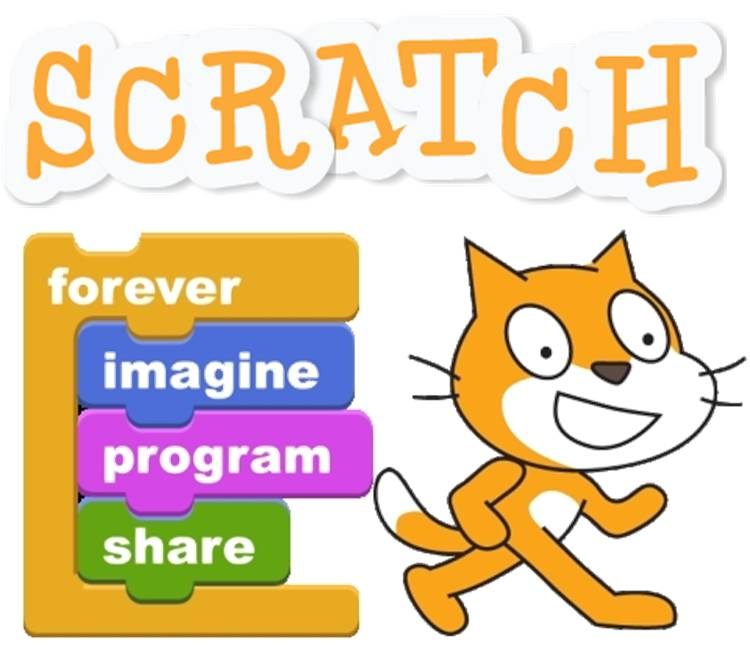
\includegraphics[width=5cm]{logoscratch.png}
    \fonte{Site do \textit{Scratch} (\textit{https://scratch.mit.edu/})}
    
\end{figure} 

O \textit{Scratch} permite desenvolver jogos, animações e textos interativos, integrando, desta forma, diversas áreas do conhecimento de forma divertida. Assim os usuários podem imaginar uma história ou um jogo e, depois de brincarem e aprenderem com a programação ainda podem compartilhar com colegas e com outros usuários da plataforma suas criações, tornando-se mais criativas e estimuladas a procurarem novas formas de resolverem problemas através da programação e do Pensamento Computacional. 

%\newpage
 
A sua interface é de fácil compreensão (vide Figura \ref{scr1}) e o uso de suas ferramentas muito intuitivas e sem complicações, possuindo três principais áreas:
 
\begin{enumerate}
\item Nesta área estão armazenados os blocos de comando, organizados a partir da sua funcionalidade.
\item A área de comandos a serem seguidos, onde os blocos serão encaixados
\item Palco ou simulador do Ecrã, onde se pode ver a simulação ou execução dos comandos.
\end{enumerate}

\begin{figure}[H]

    \center
    \caption{Interface do \textit{Scratch} \label{scr1}}
    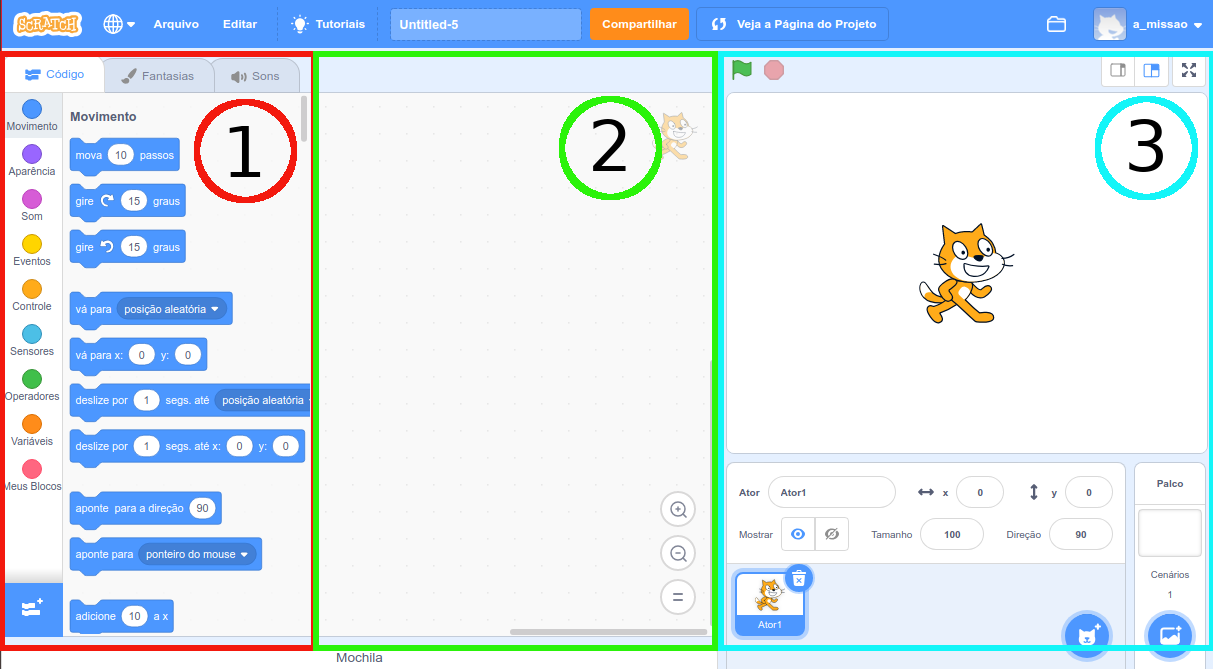
\includegraphics[width=13cm]{scratch1.png}
    \fonte{Adaptado do Site do \textit{Scratch}}
    
\end{figure}

%\newpage

A primeira área, ou área de blocos de comando (vide Figura \ref{scr2}), estão os comandos que podem ser usados na programação a ser realizada. Esses comandos estão subdivididos em categorias a partir de suas funcionalidades, como movimento, aparência, som, etc.

\begin{figure}[H]

    \center
    \caption{Área de blocos de comandos do \textit{Scratch} \label{scr2}}
    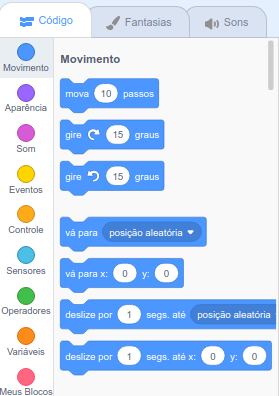
\includegraphics[height=5cm]{scratch2.png}
    \fonte{Adaptado do Site do \textit{Scratch}}
    
\end{figure}

%\newpage

Nesta área também aparecem as abas de fantasias e sons que podemos usar do próprio \textit{Scratch} ou de nossos arquivos pessoais. Note que para cada categoria de blocos de comandos existe uma legenda de cores e todos os blocos relacionados a essas categorias tem a mesma cor de suas respectivas legendas.

A segunda área, chamada área de comandos (vide Figura \ref{scr3}), é a área onde os blocos são arrastados com o mouse e encaixados de maneira lógica para formar a programação a ser seguida pelos atores escolhidos.

\begin{figure}[H]

    \center
    \caption{Área de comandos do \textit{Scratch} \label{scr3}}
    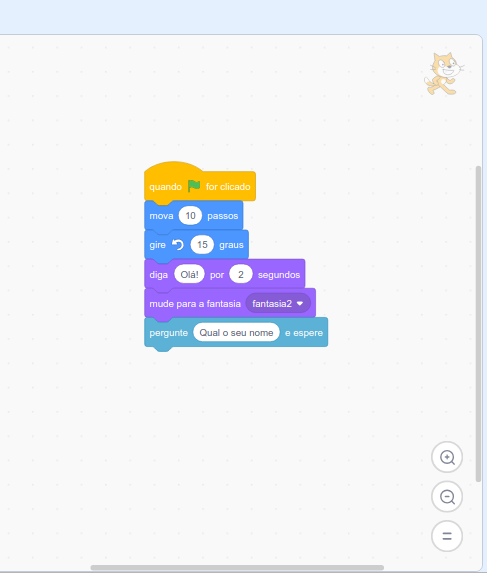
\includegraphics[height=6.3cm]{scratch3.png}
    \fonte{Adaptado do Site do \textit{Scratch}}
    
\end{figure}

É nessa área que todas as programações são montadas como um quebra-cabeça e cada ator terá sua área de comandos específica.


A terceira área (vide Figura \ref{scr4}) é onde se encontra o simulador do Ecrã (tela onde será projetada a programação), a relação dos atores e o palco com seus cenários.

\begin{figure}[H]

    \center
    \caption{Simulador de ecrã do \textit{Scratch} \label{scr4}}
    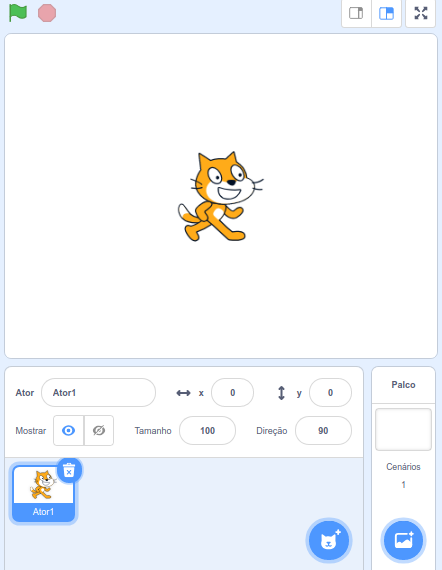
\includegraphics[height=6.3cm]{scratch4.png}
    \fonte{Adaptado do Site do \textit{Scratch}}
    
\end{figure}

O Ecrã é ``mapeado'' através de coordenadas cartesianas e o primeiro ator (também chamado de \textit{sprite}) que aparece (um gato) se posiciona inicialmente no ponto (0,0), isto é, em $x=0$ e $y=0$ e o palco apresenta-se em branco.


Por ser uma linguagem de programação, toda ação deve ser dada na forma de comandos devidamente expressos nos seus blocos lógicos que são arrastados para uma área de comandos, conectados uns aos outros ou executados através de sub-rotinas ou de subdivisões. 


 
 As suas características de linguagem de programação e de um quebra-cabeça fazem com que o \textit{Scratch} possa ser usado tanto como uma ferramenta para produção de Objetos de Aprendizagem como um meio de desenvolver o Pensamento Computacional do aluno e, em ambos os casos, esse uso poderá ser de forma interdisciplinar. Como não é necessário digitar um comando e a resposta à programação é quase que imediata, o usuário pode experimentar rapidamente o que criou e corrigir os erros caso seja necessário fazendo assim um ciclo contínuo de novas ideias, desenvolvimento, experimentação, aprendizagem e compartilhamento levando a novas ideias. 

% ?colocar exemplos de objetos de aprendizagem e de desenvolvimento de pensamento computacional?

\chapter{Metodologia do curso}

A Metodologia do curso foi desenvolvida de forma a apresentar o \textit{Scratch} como ferramenta para desenvolver objetos de aprendizagem pelo professor e também para estimulá-lo a usar este programa com os seus alunos para resolverem problemas usando o pensamento computacional como premissa. Desta forma o professor também estimula os alunos a desenvolverem habilidades relacionadas não só ao conteúdo educacional apresentado como também à construção de soluções de problemas. 

Para tanto foram realizados sete encontros com quatorze professores de modalidades de ensino e formações específicas diferentes, sendo:

\begin{itemize}

\item 4 professores que atuam na modalidade de Anos Iniciais - 1º ao 5º ano
\item 2 professores que atuam em salas de recursos para alunos com necessidades especiais
\item 4 professores que atuam na modalidade de Anos Finais - 6º ao 9º ano - sendo 3 professores de Matemática e 1 de Ciências
\item 4 professores que atuam na modalidade de Ensino Médio - 1º ao 3º ano do Ensino Médio - sendo 2 professores de Matemática e 2 de Química

\end{itemize}


Os encontros foram distribuidos de acordo com a Tabela \ref{tabcurso} abaixo: 

\begin{table}[H]
        \centering
        \caption{Planejamento do Curso sobre o \textit{Scratch} \label{tabcurso}}
        \scalebox{0.9}{        
        \begin{tabular}{ >{\centering\arraybackslash}m{2.5cm} >{\centering\arraybackslash}m{6cm} >{\centering\arraybackslash}m{6.5cm}}
            \toprule
            \textbf{Encontro} & \textbf{Conteúdo} & \textbf{Objetivo} \\
            \midrule
             \textbf{1} & Pensamento Computacional & Resolver problemas usando programação através do Pensamento Computacional como premissa \\
            \midrule
            \textbf{2} & Apresentação do \textit{Scratch}  & Ambientar os professores ao programa \\
            \midrule
            \textbf{3} & Contando Histórias & Contar uma história através da programação do \textit{Scratch} \\
            \midrule
            \textbf{4} & Programação de jogos & Desenvolver um jogo com a programação do \textit{Scratch} \\
            \midrule
            \textbf{5} & Objetos Digitais de Aprendizagem & Conhecer o que são Objetos Digitais de Aprendizagem e como utilizá-los   \\
            \midrule
            \textbf{6} & Programando Objetos Digitais de Aprendizagem & Desenvolver Objetos de Aprendizagem com o \textit{Scratch} \\
            \midrule
            \textbf{7} & Projetos desenvolvidos & Mostrar para a turma os projetos desenvolvidos com os alunos \\
            \bottomrule
        \end{tabular}
      }
       \fonte{Criado pelo autor}
    \end{table}

O curso também contou com exercícios e estudos à distância, para que os professores pudessem planejar, desenvolver e verificar a aceitação de seus alunos ao \textit{software}. Desta forma, cada professor teve a oportunidade de, ao final do curso, mostrar quais foram os problemas propostos ou como desenvolveram os programas a serem apresentados, além de mostrarem como os alunos se desenvolveram não só em suas disciplinas, como também em relação ao modo de resolverem problemas.

\section{Detalhamento dos encontros}

\begin{enumerate}[label=\textbf{\arabic*.}]

\item \textbf{Pensamento Computacional}

\end{enumerate}

Através do site \textit{https://lightbot.com/flash.html} foi introduzida a ideia de Pensamento Computacional. Neste site a pessoa tem que programar um robô através de setas e outras imagens para que ``acenda'' os blocos azuis e os transforme em amarelos (vide Figura \ref{robo2}).

\begin{figure}[H]

    \center
    \caption{ \textit{Lightbot} \label{robo2}}
    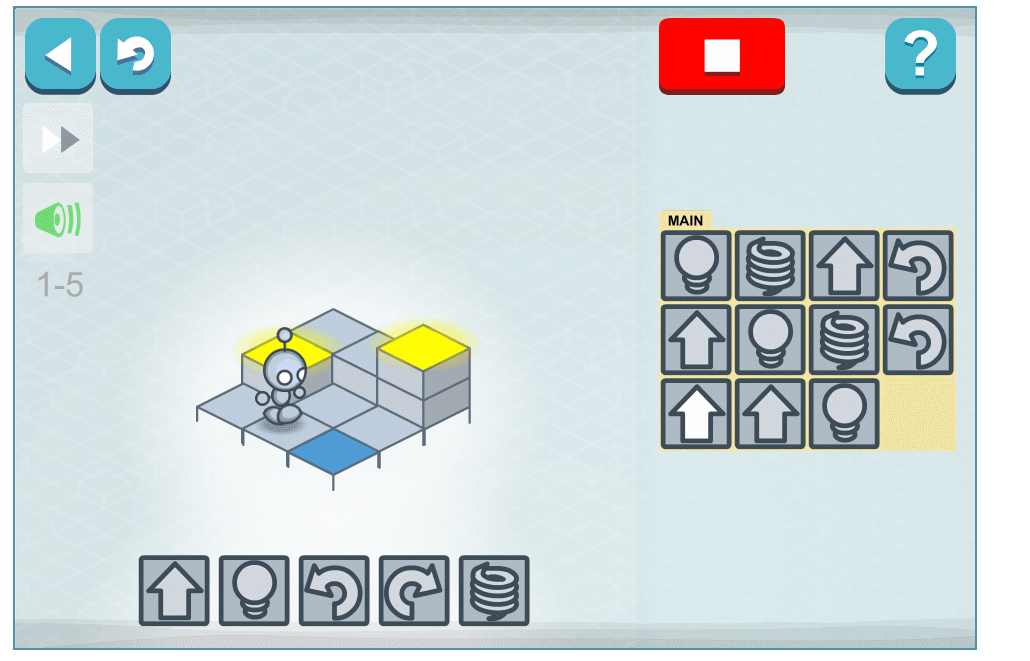
\includegraphics[height=8cm]{robo2.png}
    \fonte{https://lightbot.com/flash.html}
    
\end{figure}

É interessante notar que para que este robô acenda todos os blocos azuis, o jogador deve primeiro escolher o caminho em que o robô irá passar, dividir o caminho em pequenos blocos e escolher, dentre disponíveis, os comandos necessários e, por fim, testar a programação. Essas são características do Pensamento Computacional aplicada a um problema de caminhos.

Para melhor estruturar essas ideias, os professores leram o primeiro capítulo do artigo ``Desenvolvimento do Pensamento Computacional Através de Atividades Desplugadas na Educação Básica'' - ``Pensamento Computacional'' \cite{brac} e, desta forma, discutiram suas características e como elas também serão trabalhadas durante o curso.

\begin{enumerate}[resume, label=\textbf{\arabic*.}]

\item \textbf{Apresentação do \textit{Scratch}}

\end{enumerate}

Neste encontro os professores foram apresentados à página do \textit{Scratch} através de uma história animada construída no software (vide Figura \ref{exemploani4}) para descontrair e iniciar uma conversa sobre a computação e a sala de aula. Após esse primeiro momento foram realizados pedidos de abertura de contas especiais de professor na plataforma do \textit{Scratch}, para que, desta forma todos possam utilizar a plataforma com seus alunos. Após esse procedimento, os professores abriram pela primeira vez a área de criação de programas e fizeram seu primeiro programa escolhendo um \textit{sprite} com que mais se identificassem e, com algumas orientações de como escolher os comandos, se apresentassem através de uma história animada.



\begin{figure}[H]

    \center
    \caption{Exemplo de animação \label{exemploani4}}
    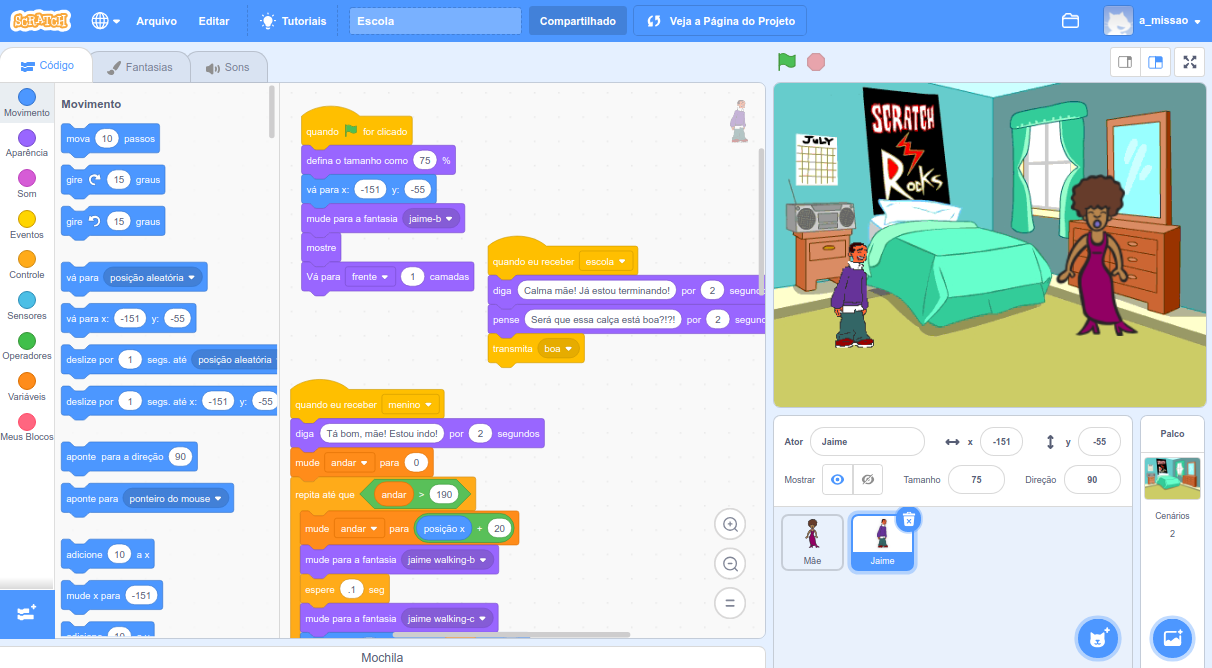
\includegraphics[height=8cm]{exemploani.png}
    \fonte{Criado pelo autor no site https://scratch.mit.edu}
    
\end{figure}
 
Ao final desse encontro, foi solicitado a cada professor que, até o próximo encontro, examinassem o conteúdo que estavam desenvolvendo em sala e observassem os seus alunos para verificar quais as dificuldades encontradas.

\begin{enumerate}[resume,label=\textbf{\arabic*.}]

\item \textbf{Contando Histórias}

\end{enumerate}


Aproveitando a ideia da pequena história desenvolvida no encontro passado, neste encontro os professores programaram histórias animadas mais elaboradas, com movimentos dos \textit{sprites} e com pausas para cada um desses personagens. Utilizaram também as trocas de cenários e de figurinos (no \textit{Scratch} chamado de fantasias) dos personagens.

Para isso, antes da programação, cada professor planejou a história a ser contada, com os diálogos que os personagens iriam desenvolver, quais os movimentos seriam necessários (dentro da capacidade do \textit{Scratch} e de cada \textit{sprite} escolhido) e em quais cenários essa história seria contada subdividindo, desta forma, a história em pequenos pedaços e assim introduzindo a ideia de criação de um pequeno algoritmo que pudesse depois ser transformado em uma programação.

Com os algoritmos prontos, pôde-se dar início a programação do \textit{Scratch}, utilizando principalmente os conjuntos de comandos de movimento, de aparência (onde se encontram os comandos de fala escrita), de eventos e de controle.

Ao fim do encontro, para a fase à distância, os professores desenvolveriam uma história a ser contada através do \textit{Scratch} para os alunos e também mostrar-lhes como desenvolver as suas próprias histórias animadas.

\begin{enumerate}[resume,label=\textbf{\arabic*.}]

\item \textbf{Programação de jogos}

\end{enumerate}

Para a melhor compreensão de como desenvolver um jogo, de forma dirigida e conjunta, todos os professores construiram um algoritmo em que um \textit{sprite} pudesse ``flutuar'' no ecrã do \textit{Scratch}. Considerando esse algoritmo desenvolvido em conjunto como apenas uma base de vários jogos, cada professor poderá escolher como o seu jogo será apresentado, escolhendo cenários e  personagens distintos mas com a mesma movimentação inicial. Por exemplo, o cenário pode ser  o fundo do mar e o personagem um mergulhador ou então o cenário pode ser o céu de uma cidade e o personagem uma ave, nestes dois casos o movimento de ``flutuar'' será o mesmo mas os obstáculos apresentados para cada personagem criarão jogos diferentes entre si, com objetivos também diferentes.

Ao escolherem os personagens e o cenário, o jogo começa a ficar mais pessoal, e assim o restante do algoritmo e dos objetivos dos jogos serão escritos de forma mais individual.

A transformação desse algoritmo em uma programação do \textit{Scratch} foi realizada utilizando os conjuntos de comandos utilizados no encontro anterior juntamente com os conjuntos de sensores, operadores e variáveis disponíveis.



\begin{enumerate}[resume,label=\textbf{\arabic*.}]

\item \textbf{Objetos Digitais de Aprendizagem}

\end{enumerate}

O quarto encontro teve como objetivo principal o estudo e o primeiro esboço de um Objeto Digital de Aprendizagem a ser desenvolvido pelos professores de acordo com suas disciplinas e conteúdos, levando em conta as dificuldades observadas em sala de aula, e, quando pronto, apresentado aos alunos.

Em um primeiro momento, os professores tiveram contato com um jogo desenvolvido com o objetivo de praticar os conceitos de soma e subtração de números naturais restringidos até o número 10 entre as parcelas (vide Figura \ref{somaesub}). Desta forma eles puderam ver como elaborar um Objeto Digital de Aprendizagem com o \textit{Scratch}.

\begin{figure}[H]

    \center
    \caption{Jogo Soma e Subtração \label{somaesub}}
    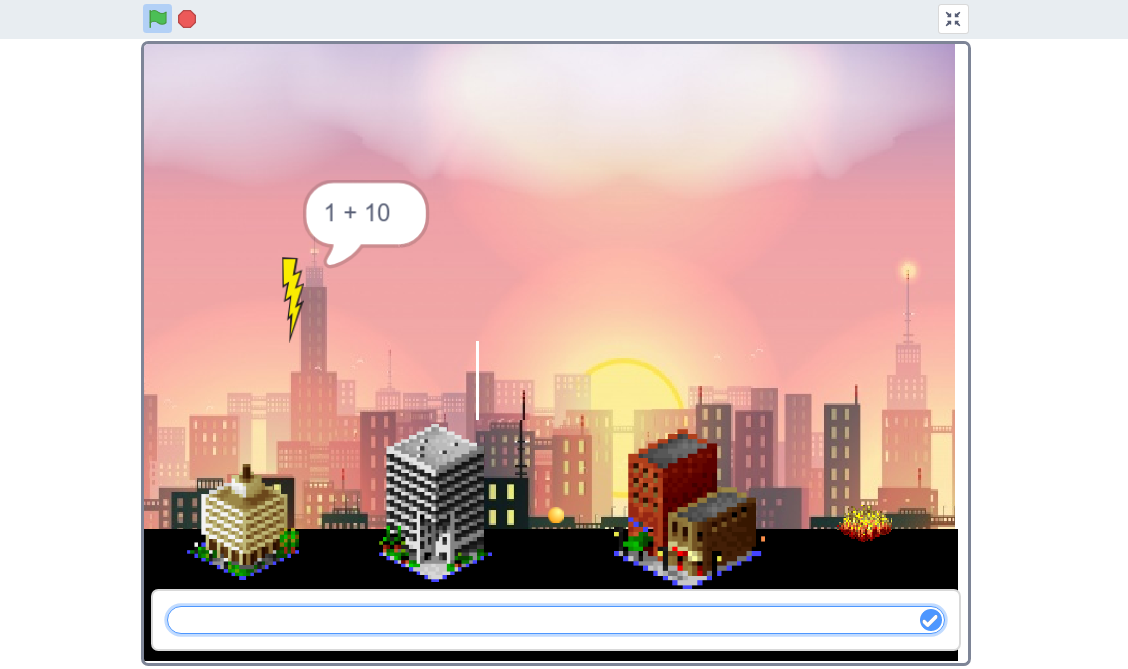
\includegraphics[height=8cm]{somaesub.png}
    \fonte{Criado pelo autor no site https://scratch.mit.edu}
    
\end{figure}


Após o jogo os professores leram e discutiram em grupos de no máximo 3 pessoas o primeiro capítulo do livro ``Objetos de aprendizagem: Teoria e prática'' - ``Objetos de aprendizagem: Conceitos Básicos'' \cite{tarouco} e, após essa discussão, começaram a delinear, cada um, um projeto de Objeto Digital de Aprendizagem que pudessem desenvolver no \textit{Scratch} e para a fase à distância, eles ficaram com a incumbência de escrever um algoritmo que pudesse detalhar todos os momentos desse Objeto seja ele uma história, um jogo ou qualquer outra ideia que tivessem delineado neste encontro.

\begin{enumerate}[resume,label=\textbf{\arabic*.}]

\item \textbf{Programando Objetos Digitais de Aprendizagem}

\end{enumerate}

Com os algoritmos prontos, os professores programaram, através de novas orientações de quais comandos estavam à disposição e como funcionam sub-rotinas no \textit{Scratch}, caso fossem necessárias, os seus Objetos Digitais de Aprendizagem através do \textit{Scratch}, tendo como objetivo, apresentar aos seus alunos na próxima fase à distância. Desta forma, todos puderam perceber como se estrutura, na prática, uma programação e também como fazer um Objeto de Aprendizagem voltado para as necessidades específicas de cada professor, de cada conteúdo e o mais importante, de cada aluno que irá usá-lo.

A fase à distância desse encontro foi apresentar aos alunos os Objetos Digitais de Aprendizagem desenvolvidos por eles e fazer uma nova observação da aceitação desta ferramenta e como foi o desenvolvimento da aprendizagem de cada aluno.

\begin{enumerate}[resume,label=\textbf{\arabic*.}]

\item \textbf{Projetos desenvolvidos}

\end{enumerate}

Este encontro foi planejado para que cada professor apresente os projetos desenvolvidos por eles e pelos seus alunos. Além dessa apresentação, os professores fizeram considerações sobre como cada aluno percebeu os Objetos Digitais de Aprendizagem desenvolvidos e como esses mesmos alunos desenvolveram os seus próprios programas dentro da plataforma, utilizando-a para contar histórias, para elaborar jogos, ou mesmo para resolver problemas elaborados pelo professor através da programação.

\section{Principais projetos desenvolvidos}

Para uma melhor organização dos principais projetos e o entendimento do contexto dos resultados, esse tema foi dividido em três momentos importantes do curso: O primeiro contato dos alunos com a plataforma através do desenvolvimento de histórias animadas, a produção de Objetos Digitais de Aprendizagem pelos professores e a utilização do \textit{Scratch} pelos alunos no desenvolvimento de jogos ou de programas através de problemas propostos.

A primeira atividade dos professores com seus alunos, o desenvolvimento da história animada, teve uma ótima repercussão entre os professores que além de contarem algumas histórias para seus alunos, puderam perceber como seus alunos podem interagir com essas histórias. Os professores de anos iniciais juntaram-se em grupo e usaram estas histórias como forma de fixação de leitura e interpretação de texto, já que alguns de seus alunos acabaram de ser alfabetizados e estavam ainda tendo dificuldades em compreender o que estavam lendo. Os que tinham mais facilidade em interpretação de texto, segundo os professores, se motivaram a também escreverem histórias e as estavam desenvolvendo tanto no site do \textit{Scratch} como em forma de quadrinhos em seus cadernos. Os professores que atuavam em salas de recursos usaram outras abordagens para contar suas histórias, usando estímulos como sons de animais e objetos que encontraram em \textit{sites} de efeitos sonoros para desenvolver uma melhor interação com os seus alunos.

Os resultados mais significativos desse primeiro contato com os alunos vieram dos relatos dos professores que atuam nos Anos Finais e no Ensino Médio, pois seus alunos foram estimulados a contar as suas próprias histórias dentro da plataforma. Para melhor direcionar essas histórias, os professores foram orientados que pedissem aos alunos para pesquisar um fato histórico ou um personagem relacionado ao conteúdo trabalhado em sala. Desta forma a programação dessa história envolveu outras disciplinas e motivou os alunos a aprenderem o conteúdo e também a representá-lo. 

Dentre esses trabalhos o que mais se destacou foi desenvolvido pelo professor de Ciências na modalidade Anos Finais, cujo conteúdo foi a ``História da Física'': Os seus alunos foram separados em grupos e escolheram os personagens históricos que desenvolveram a Física como Ciência. Pesquisaram quais as contribuições desses personagens e transformaram essa narrativa em uma programação no site do \textit{Scratch}. Usando como exemplo a história de Aristóteles narrada por um destes alunos e analisando a programação realizada, pode-se perceber como esta programação envolve várias disciplinas (vide o conjunto de Figuras \ref{histaris}).

\begin{figure}[H]

 \centering
 
         \caption{Programação da História de Aristóteles \label{histaris}}
     \begin{subfigure}[b]{0.3\textwidth}
         \centering
         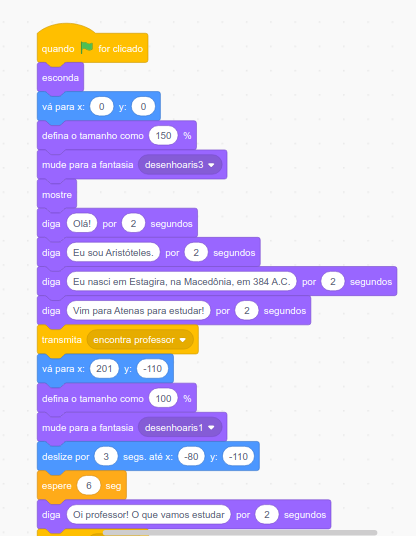
\includegraphics[height=8cm]{histaristoteles1.png}
         \caption*{Aristóteles}
         \label{aristoteles}
     \end{subfigure}
     \hfill
     \begin{subfigure}[b]{0.3\textwidth}
         \centering
         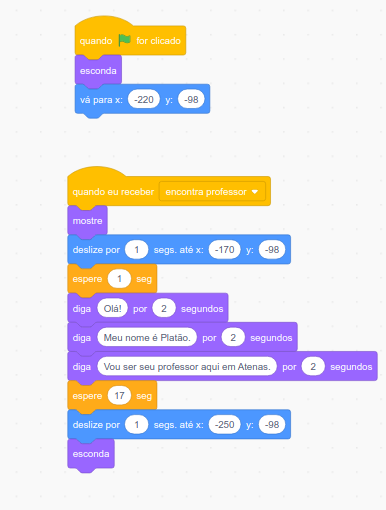
\includegraphics[height=8cm]{histaristoteles3platao.png}
         \caption*{Platão}
         \label{platao}
     \end{subfigure}
     \hfill
     \begin{subfigure}[b]{0.3\textwidth}
         \centering
         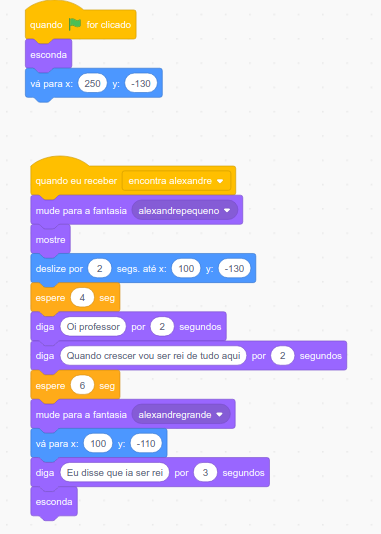
\includegraphics[height=8cm]{histaristoteles2alexandre.png}
         \caption*{Alexandre}
         \label{alexandre}
     \end{subfigure}
     
     \fonte{https://scratch.mit.edu/projects/378647189/}
    
\end{figure}

Envolvendo a disciplina de História, o aluno usou três personagens: Platão, Alexandre e o próprio Aristóteles. No campo da Matemática, a primeira aparição de Aristóteles aparece um pouco maior que no restante da narrativa, e vemos na programação que o aluno usou a ideia de porcentagem para este aumento e, além disso, para posicioná-lo usou o sistema do Ecrã do \textit{Scratch}, que é baseado no Plano Cartesiano. Em Filosofia, usou os pensamentos filosóficos da época para mostrar como foram as contribuições de Aristóteles para a Física, para a Óptica e para a própria Filosofia. Ainda temos o estudo da Língua Portuguesa, que perpassa por toda a história, tanto na narração como nos diálogos dos personagens. 

Após esse primeiro momento, os professores desenvolveram Objetos Digitais de Aprendizagem para apresentar aos alunos. 

Os professores que atuavam em salas de recurso desenvolveram dois programas para ajudar os alunos que tinham dificuldades motoras e não conseguiam ter o domínio do \textit{mouse}. 

O primeiro programa (vide Figura \ref{rec1}) foi desenvolvido para que o aluno pudesse movimentar uma bola que flutuava e mudava de cor ao encostar em algum elemento no palco.

\begin{figure}[H]

 \centering
 
         \caption{Palco e Programação da bola que muda de cor \label{rec1}}
         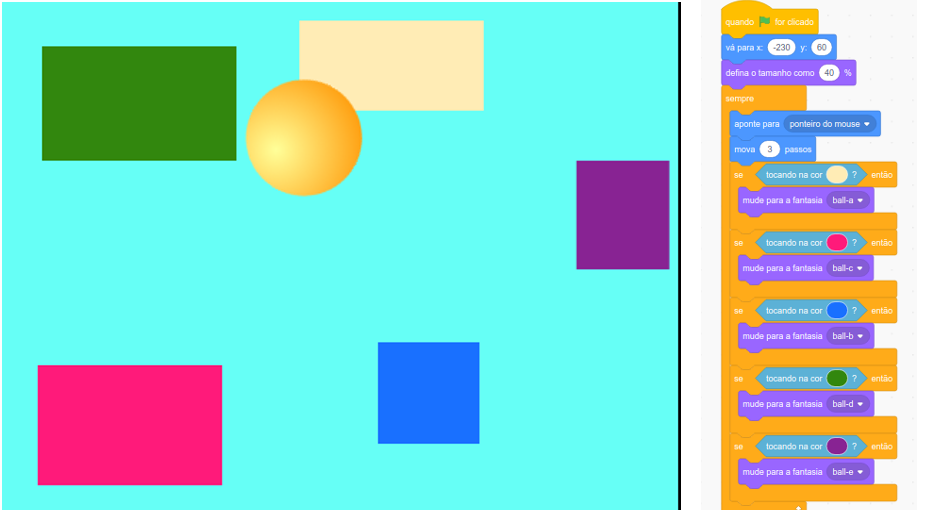
\includegraphics[height=8.5cm]{progcorbola.png}
     \fonte{https://scratch.mit.edu/projects/333029656/}
    
\end{figure}

O segundo programa tinha como objetivo conduzir uma bola com o mouse até o buraco através de um caminho não podendo tocar nas bordas do caminho.


\begin{figure}[H]

 \centering
 
         \caption{Palco da Condução de bola \label{palcorec2}}
     
         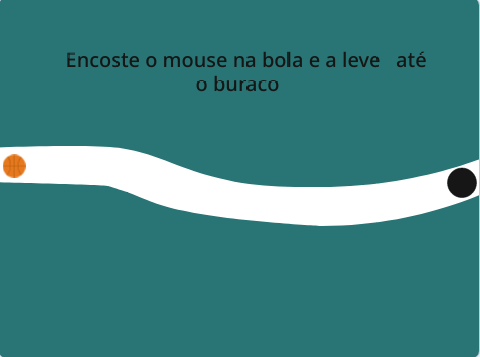
\includegraphics[height=4.5cm]{palcorec22.png}
        
 
     \fonte{https://scratch.mit.edu/projects/400103790/}
    
\end{figure}

Esses professores de sala de recursos desenvolveram esses projetos para alunos com necessidades especiais de movimentos com o objetivo de ajudá-los a adquirir uma melhor coordenação motora para o uso do computador não só como meio de comunicação e informação, mas também como ferramenta de aprendizagem, já que ao conseguir manusear o mouse, este aluno terá capacidade de usar programas e aplicativos no computador com mais independência.

Um outro Objeto Digital de Aprendizagem relevante foi desenvolvido por um professor de Química para o Ensino Médio. 


\begin{figure}[H]

 \centering
 
         \caption{Palco do \textit{Quiz} Reações e Balanceamento \label{quiz}}
     
         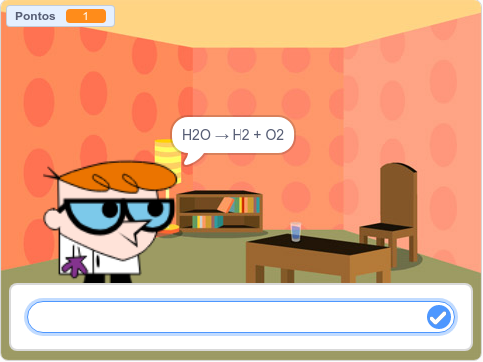
\includegraphics[height=7cm]{quimicatela.png}
        
 
     \fonte{https://scratch.mit.edu/projects/334853158/}
    
\end{figure}

Este é um jogo em que o aluno interage com o personagem através de perguntas e respostas sobre quais são os tipos de equações químicas e qual o balanceamento correto em determinadas equações. Ao iniciar, o aluno escolhe uma entre duas opções: Distinguir qual é o tipo de equação que irá aparecer ou fazer o balanceamento de alguma equação. Este projeto foi desenvolvido com a premissa de que o aluno já tenha conhecimento do que é balanceamento e dos tipos de reações químicas e, com essas perguntas e respostas, ele pode fixar esses conceitos.

Os professores mostraram interesse maior em produzir seus próprios Objetos Digitais de Aprendizagem pois, desta forma, poderiam focar essas produções em conteúdos mais complexos ou em dificuldades específicas de cada aluno. Observou-se também que o professor começou a sentir-se mais seguro não só com o \textit{Scratch} mas também com as suas produções, porque, como são autorais, pode ser melhor administrada pelo autor e o seu conteúdo pode estar mais próximo do que é desenvolvido em sala de aula.

O terceiro momento do curso consistia em incentivar os alunos a desenvolverem seus próprios algoritmos e programas. Mesmo sendo o objetivo principal o estudo dos conteúdos desenvolvidos dentro de sala de aula, os alunos poderiam construir jogos, criar animações, histórias ou qualquer outro programa que envolvesse esse conteúdo. Para tanto, os professores poderiam elaborar situações problemas ou propor aos alunos alguma outra forma de estudo a ser transformada em programação.

Dentre as situações problemas propostas, destaca-se o trabalho realizado pelos professores de Matemática dos Anos Finais relacionado a razão e proporção. O problema consistia em saber qual a quantidade de cada um dos ingredientes necessários para fazer uma determinada receita. Para desenvolverem os programas, os alunos foram separados em grupos e cada grupo escolheu uma receita para ser estudada. Um dos programas desenvolvidos calcula a quantidade de ingredientes necessários para fazer pão.

\begin{figure}[H]

 \centering
 
         \caption{Palco e Programação da Receita de Pão \label{pao}}
         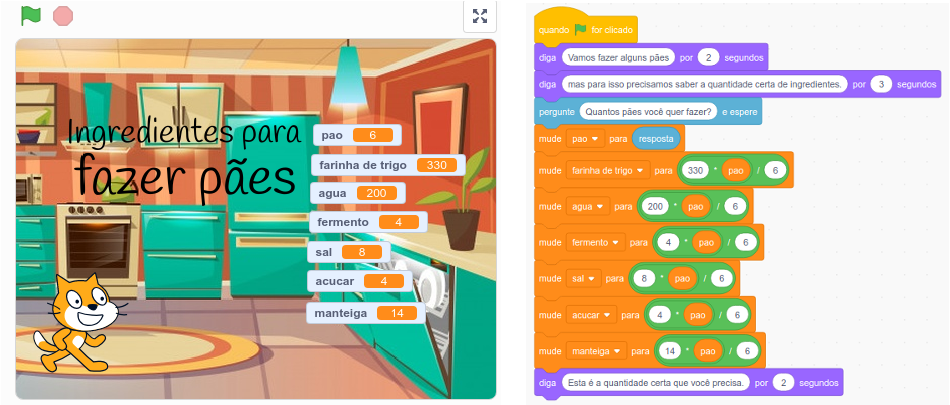
\includegraphics[height=7cm]{recpao.png}
       
     \fonte{https://scratch.mit.edu/projects/401180286/}
    
\end{figure}


Neste programa (vide Figura \ref{pao}), a pessoal informa qual a quantidade de pães quer fazer e o programa calcula a quantidade de ingredientes necessários para a receita. 

Mesmo com uma programação simples e com poucos comandos, percebe-se como o aluno usou os conceitos de desenvolvimento do Pensamento Computacional apresentados. Em primeiro lugar, houve uma coleta dos dados iniciais, onde o aluno pesquisou quais ingredientes eram necessários para a produção de certa quantidade de pães. Após a coleta de dados, analisou a quantidade de cada um dos ingredientes e, através de cálculos envolvendo proporção, automatizou soluções por meio de pensamento algorítmico, generalizando estas quantidades de ingredientes para qualquer quantidade de pães necessários. Para chegar a essa solução, o aluno não só usou as regras de proporção, que era o conteúdo inicial a ser estudado, mas também aprendeu a pesquisar e a analisar os textos da receita.

Um segundo trabalho produzido por alunos de anos iniciais a ser destacado é um jogo de tabuleiro que envolve um questionário estimulado pelo professor de Ciências. Envolvendo dois jogadores, o objetivo é chegar ao final do tabuleiro com a ajuda de um dado virtual e, em se parando em determinados lugares, o jogador deverá responder a uma pergunta envolvendo conhecimentos sobre \textit{Misturas Homogêneas e Heterogêneas} e sobre \textit{Estados Físicos da Matéria} (vide Figura \ref{tabule}).

\begin{figure}[H]

 \centering
 
     \caption{Palco do jogo de Tabuleiro \label{tabule}}
     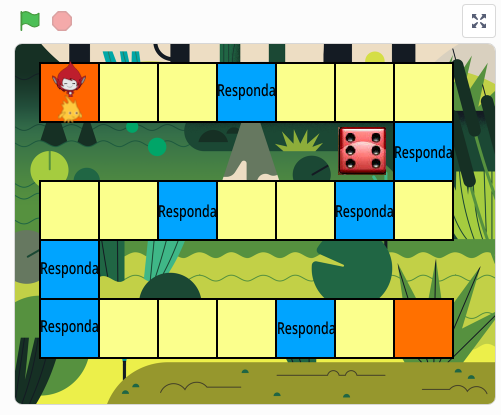
\includegraphics[height=6.5cm]{palcotabuleiro.png}
       
     \fonte{https://scratch.mit.edu/projects/403307051/}
    
\end{figure}

Para este jogo foram utilizados três \textit{Sprites} (personagens) programáveis: dois que representam os jogadores e o dado que é usado para o movimento no tabuleiro. Ao analisar a programação de cada um desses personagens, pode-se perceber características interdisciplinares relevantes além do conteúdo trabalhado diretamente pelo professor de Ciências.

A programação do dado inclui porcentagem, localização em um plano cartesiano e, apesar de ainda não calcular probabilidades, o aluno já tem contato com números e experimentos aleatórios (vide Figura \ref{dado})

\begin{figure}[H]

 \centering
 
     \caption{Programação do dado \label{dado}}
     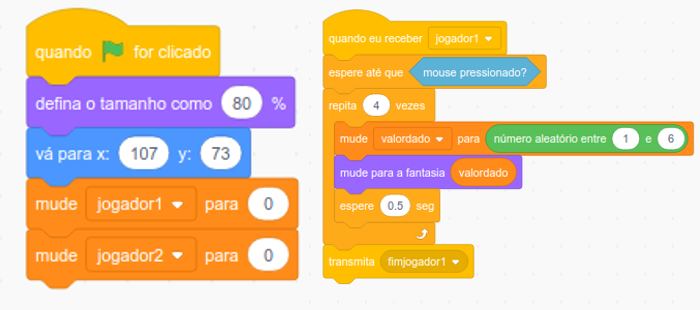
\includegraphics[height=5.5cm]{dadofinal.png}
       
     \fonte{https://scratch.mit.edu/projects/403307051/}
    
\end{figure}

A programação dos outros dois personagens além de incluir porcentagem e localização no plano cartesiano, tem também a movimentação nos eixos $x$ e $y$ do plano usando números positivos e negativos para orientar em qual direção esses personagens irão se movimentar (vide Figura \ref{progtab}).

\begin{figure}[H]

 \centering
 
     \caption{Programação dos participantes \label{progtab}}
     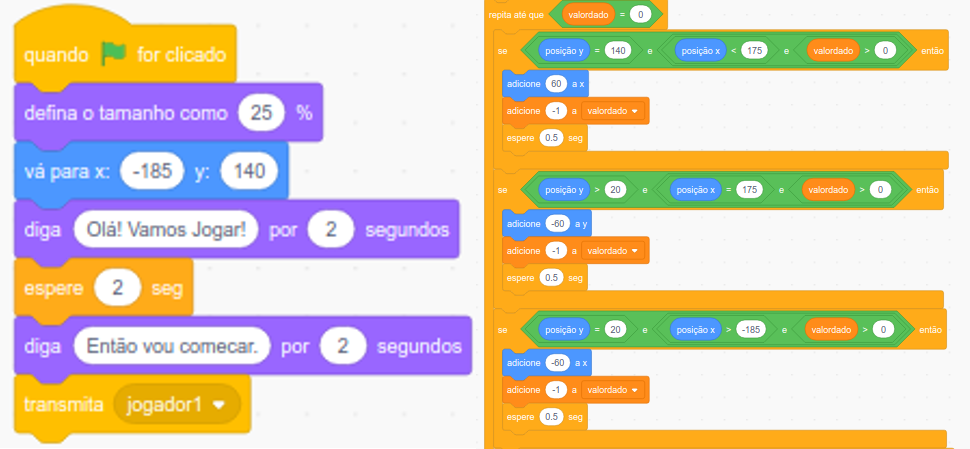
\includegraphics[height=7cm]{progtabfinal.png}
       
     \fonte{https://scratch.mit.edu/projects/403307051/}
    
\end{figure}

Existe também a inserção dos conteúdos de Ciências estudados na pesquisa das perguntas formuladas e suas respostas durante a movimentação dos personagens. Desta forma, o aluno, além de ser estimulado a criar um jogo autoral, adquiriu habilidades que seriam mais complexas para o seu nível de desenvolvimento, onde o professor desempenhou o papel de orientar esse progresso.



\chapter{Conclusão}
% \addcontentsline{toc}{chapter}{Conclusão}


O \textit{Scratch} se mostra uma ferramenta importante quando se busca por novas abordagens de educação mediada pelo uso das novas Tecnologias Digitais de  Informação e de Comunicação de forma interdisciplinar onde o aluno é alçado a protagonista. Quando o aluno é estimulado a pensar de forma lógica e a resolver problemas através da linguagem de programação, a sua capacidade de abstrair e de fazer relações entre diversos conteúdos e conhecimentos também é estimulada e, além disso, o professor também é influenciado a se tornar cada vez mais um orientador em vez de um detentor de conhecimentos.

Mas de nada adianta ferramentas como essa estarem disponíveis se o professor não conhecer as suas potencialidades e também não for estimulado a usá-las. Foi o que se percebeu no início do curso, quando alguns professores se mostraram receosos ao serem apresentados à ideia de inserir a computação em sua prática pedagógica. Esses professores tinham a percepção de que a programação só poderia ser pensada e realizada através de comandos rebuscados dentro de uma linguagem de máquina, por isso foi importante, logo no primeiro encontro, apresentar o \textit{lightbot}, mostrando que a programação está mais ligada ao desenvolvimento de um pensamento lógico e a resolução de problemas do que à linguagens específicas. Mesmo após esse início, alguns só conseguiram se motivar mais e a aprender um pouco mais sobre como usar o Pensamento Computacional após serem apresentados realmente ao \textit{Scratch} e fazerem a sua primeira historinha para se apresentarem, percebendo que a programação pode ser um fator de desenvolvimento do pensamento lógico e abstrato dos alunos.

O primeiro momento em que os alunos foram estimulados a utilizar a plataforma seja para acompanhar ou para criar uma história, foi quando os professores já conseguiam fazer as suas próprias histórias. Os alunos se motivaram a aprender mais sobre a programação de seus personagens e de suas histórias, de forma a conseguirem organizar os pensamentos e a planejar melhor as suas próximas ações. Essa empolgação do alunos em suas primeiras programações, fizeram com que os professores também ficassem animados e receptivos para o segundo momento importante do curso, que foi a construção de objetos digitais de aprendizagem, que requereu dos professores um pouco mais de planejamento. Para construir seus Objetos Digitais de Aprendizagem os professores pesquisaram, através das dificuldades de seus alunos, quais conteúdos deveriam estar inseridos, desenvolveram algoritmos que expressavam como deveriam funcionar e fizeram a programação. Todo esse planejamento e desenvolvimento de objetos os ajudou a perceber como deveriam orientar os seus alunos para que estes pudessem construir seus próprios programas.

Através dos relatos dos professores durante a apresentação dos projetos desenvolvidos no último encontro, percebeu-se que, quando os alunos foram incentivados a desenvolverem jogos, histórias ou até mesmo a resolverem pequenos problemas através do \textit{Scratch}, a postura dos professores foi mudando gradativamente, deixando de ser os detendores do conhecimento e passando a ser orientadores, facilitando a criação, a independência, o raciocínio lógico e a aprendizagem desse aluno. Além disso os alunos estavam deixando de ser apenas usuários da tecnologia e passavam a ser criadores e desenvolvedores, interagindo com essas tecnologias de forma a produzir novos conhecimentos de forma interdisciplinar e conectada com as informações que estão dispostas ao seu redor.

Desta forma, o \textit{Scratch} mostra-se tanto como uma plataforma de aprendizagem interdisciplinar oferecendo ao aluno novos conhecimentos e habilidades, como também pode ser usado para inserir os princípios do Pensamento Computacional em sala de aula, trazendo novas perspectivas à aprendizagem e à relação entre professores e alunos e à relação entre o aluno e as tecnologias.


%novas configurações

\bookmarksetup{startatroot}% 
% ---

% ---
% Conclusão
% ---

%\lipsum[31-33]

% ----------------------------------------------------------
% ELEMENTOS PÓS-TEXTUAIS
% ----------------------------------------------------------
\postextual

%---------------------------------------------------------------------
% INDICE REMISSIVO
%---------------------------------------------------------------------

%anexo de apendices

\bibliography{bibliografia}

\begin{comment}

\begin{apendicesenv}
\partapendices

\chapter{Tutorial Scratch}

Esse tutorial foi desenvolvido com base na versão online de Maio de 2020 do \textit{Scratch} que pode ser acessado em seu site oficial desenvolvido pelo \textit{Massachusetts Institute of Technology} (MIT), \textit{https://scratch.mit.edu}.

\section{Tela Inicial}

Ao abrir o \textit{site}, a primeira tela a aparecer é a tela de boas vindas:

\begin{figure}[H]

    \center
    \caption{Tela de boas vindas \label{boasvindas}}
    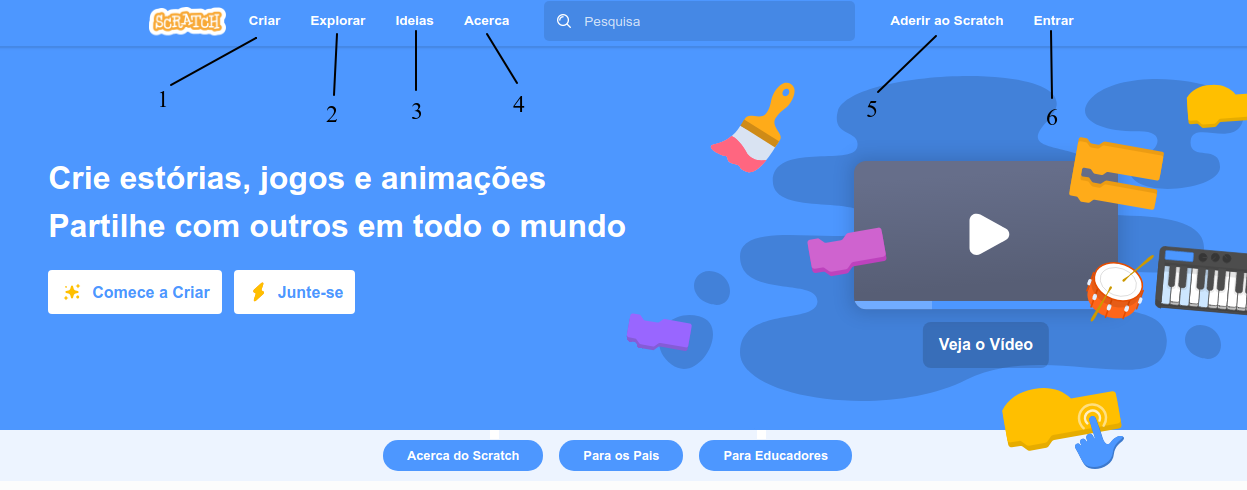
\includegraphics[height=6.5cm, width=15cm]{boasvindasscratch.png}
    \fonte{Adaptado pelo autor do site https://scratch.mit.edu}
    
\end{figure} 

Nesta tela, os principais \textit{links} que aparecem são:

\begin{table}[H]
        \centering
        \caption{Links da tela de boas vindas \label{tabboasvindas}}
                
        \begin{tabular}{ >{\centering\arraybackslash}m{3cm} >{\centering\arraybackslash}m{5.5cm} >{\centering\arraybackslash}m{6cm}}
            \toprule
            \textbf{N${}^o$} & \textbf{\textit{LINK}} & \textbf{DIRECIONAMENTO} \\
            \midrule
            \textbf{1} & Criar  & Tela de edição \\
            \midrule
            \textbf{2} & Explorar & Projetos compartilhados \\
            \midrule
            \textbf{3} & Ideias & Ideias para começar a programar \\
            \midrule
            \textbf{4} & Acerca & Apresentação do \textit{Scratch} \\
            \midrule
            \textbf{5} & Aderir ao Scratch & Inscrever-se no \textit{site} \\
            \midrule
            \textbf{6} & Entrar & Fazer \textit{login} no site \\
            \bottomrule
        \end{tabular}
        \fonte{Criado pelo autor}
    \end{table}
    
Observe que o usuário pode começar a criar mesmo sem fazer \textit{login} na plataforma.

\section{Tela de Programação}

Para uma melhor entendimento, separamos os campos principais da tela de programação:

\begin{figure}[H]

    \center
    \caption{Tela de Programação \label{telaprogramacao}}
    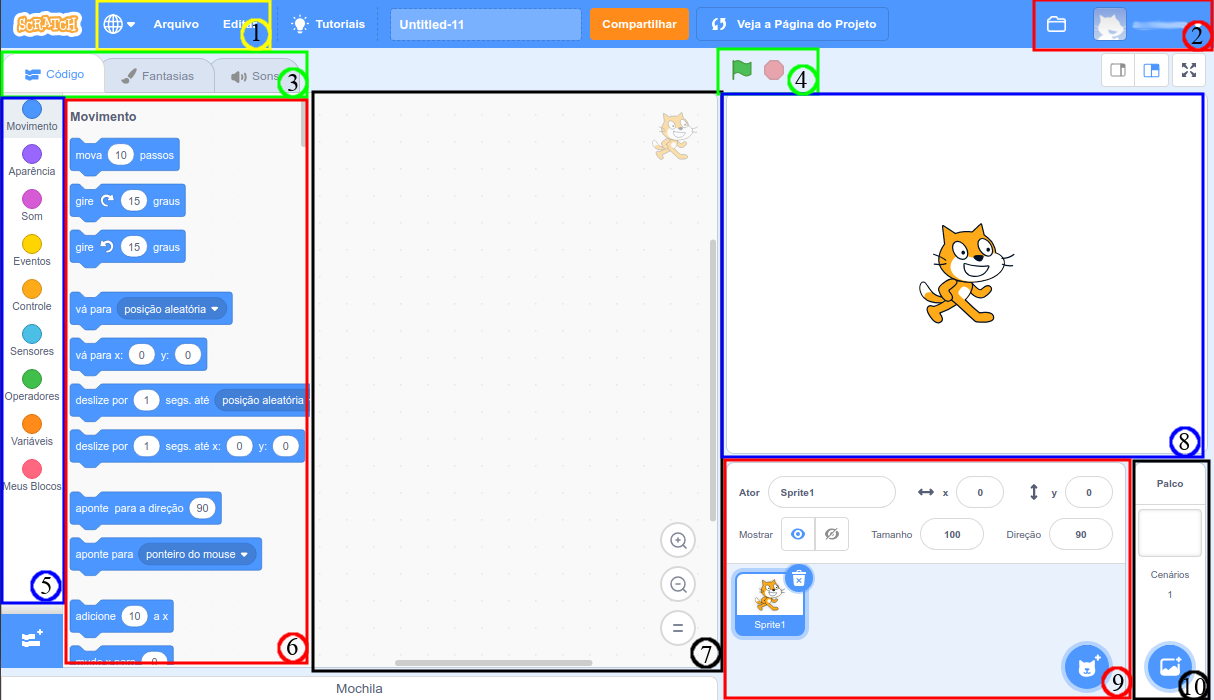
\includegraphics[height=8cm]{teladeedicao2.png}
    \fonte{Adaptado pelo autor do site https://scratch.mit.edu}
    
\end{figure} 

\begin{enumerate}

\item Menus do programa;
\item Ferramentas do usuário;
\item Paleta de acesso aos Códigos, Fantasias e Sons;
\item Botões de início e de interrupção do programa;
\item Categorias dos comandos;
\item Blocos de comandos;
\item Área de programação;
\item Palco;
\item Área de configuração e escolha dos \textit{Sprites} (personagens);
\item Área de configuração do palco e escolha dos cenários

\end{enumerate}


\end{apendicesenv}

\end{comment}
%Linha na nova configuração

\printindex





\end{document}